%% This is an example using the fubcsdiss.cls.
%%
%% Author: Marco Vervoort, ILLC UvA
%% Modified by: Marijke Keet, KRDB FUB
%%
%% Version: December, 2007.
%%
%%
%%
%%
\documentclass{fubcsdiss}

%If you use Latex2.09 instead of Latex2e, comment the \documentclass line
%and uncomment one of the following lines (depending on whether you
%also want to use MakeIndex)

%\documentstyle[12pt,epsf]{illc_diss}
%\documentstyle[12pt,makeidx,epsf]{illc_diss}

%If you want to use MakeIndex, uncomment these lines
%\usepackage{makeidx}     % only with Latex2e
%\makeindex

%%%%%%%%%%%%%%%%%%%%%%%%%%%%%%%%%%%%%%%%%%%%%%%%
% put your list of packages here with \usepackage{}. several nifty ones for customization options are commented out below and annotated, merely as suggestion.

%\usepackage{natbib} % for funky \cite options

\usepackage{amsmath}
\usepackage{mathenv}
\usepackage{amssymb}
\usepackage{amsthm}
\usepackage{graphicx}
\usepackage{textcomp}
 \usepackage{longtable} %table spanning pages
\usepackage{multirow}
% \usepackage{lscape} % for landscape pages
\usepackage{pifont}
\usepackage[font=small,labelfont=it,bf]{caption} %for customizable figure and table captions

% \usepackage{fancyhdr}  % you can choose between 7 different types of heading, besides the default. for instance, try 
%\usepackage[Lenny]{fncychap} 
% or \usepackage[Bjarne]{fncychap} % or Sonny, or Conny
%\usepackage[Sonny]{fncychap} 

%\usepackage{algorithmic}
%\usepackage{algorithm}
\usepackage{listings}
\usepackage{xspace}
% \usepackage{palatino} %for different font type
% \usepackage[T1]{fontenc}
%\usepackage[scaled]{uarial}% for the modern-look fonttype:
%\renewcommand*\familydefault{\sfdefault}

%\usepackage{soul, color} % this with the next one gives convenient colouring options for drafts, e.g. with a \hl{xxx}, the marking becomes ugly green.

%\sethlcolor{green} 
%\setul{2pt}{0.5pt} % use this if you want to change spacing of the underling

 \usepackage[neveradjust]{paralist} %this one is handy if you are short on space or want to have a listing with bulletes, starts etc. e.g. use \begin{compactenum} \item ... \end{comactenum}

%\usepackage[top=3cm, bottom=2.8cm, left=2.7cm, right=2.7cm]{geometry} % to make nice page margins to squezze more or less text on a page

%%%%%%%%%%%%%%%%%%%%%%%%%%%%%%%%%%%%%and then my shortcuts

% put your \newcommand etc here. For instance, the following formats are quite nice, but you also can take the default by commenting them:

\newtheorem{lem}{\textsc{Lemma}}[chapter]
\newtheorem{thm}{\textsc{Theorem}}[chapter]
\newtheorem{prop}{\textsc{Proposition}}[chapter]
\newtheorem{post}{Postulate}[chapter]
\newtheorem{corr}{\textsc{Corollary}}[chapter]
\newtheorem{defs}{\textsc{Definition}}[chapter]
\newtheorem{cons}{\textsc{Constraint}}[chapter]
\newtheorem{ex}{\textbf{Example}}[chapter]
\newtheorem{qu}{\textbf{Question}}[chapter]

%\makeindex

%\typeout{FUB CS Dissertation Example File `guide.tex' <June 23, 2007>.}

%%%%%%%%%%%%%%%%%%%%%%%%%%%%%%%%%%%%%%%%%%%%%%%%%%%%%%%%%

\begin{document}

 \pagestyle{plain}
\pagenumbering{roman}

%%%%%%%%%%%%%%%%%%%%%%%%%%

%%  \include the `front matter'

%% This is the standard `front matter' to be used with the illcdiss.cls
%% Latex2e document class or the illc_diss.sty Latex2.09 style file
%%
%%
%% MAKE SURE THAT THE FILE HAS BEEN PERSONALIZED BEFORE YOU
%% PRINT AND SHIP THE FINAL VERSION.  YOU CAN FIND ITEMS THAT NEED
%% TO BE PERSONALIZED BY SEARCHING FOR THE STRING ``%PERSONALIZE''
%%
%%
%%first of all the cover.
{\pagestyle{empty}
\newcommand{\printtitle}{%
{\Huge\bf The FUB-CS Dissertation\\[0.8cm] Style}}    %PERSONALIZE

\begin{titlepage}
\par\vskip 2cm
\begin{center}
\printtitle
\vfill
{\LARGE\bf John B. Goode}                           %PERSONALIZE
\vskip 2cm
\end{center}
\end{titlepage}
%
% Skip a page to start on a right page again.
% If you're printing single-sided, simply delete    %PERSONALIZE
% the following line.
%

\mbox{}\newpage
\setcounter{page}{1}

%%the very first page: the `franse pagina'
\par\vskip 2cm
\begin{center}
\printtitle
\end{center}

%%the second page: the `FUB-CS pagina'
\clearpage
\par\vskip 2cm
\begin{center}
\par\vspace {1cm}
\fubcslogo{10cm}
\par\vspace {2cm}
\textbf{FUB-CS Dissertation Series DS-2009x-NN}   %PERSONALIZE                
\par\vspace {7cm}
\noindent%

Per ulteriori informazioni sulle pubblicazioni della LUB, si prega di contattare \\
\emph{F\"{u}r weitere Informationen \"{u}ber FUB Publikationen, bitte wenden Sie sich an}\\
For further information about FUB-CS publications, please contact\\
\begin{table}[!h]
	\centering
		\begin{tabular}{p{5cm}lll}
Facolt\`{a} di Scienze e Tecnologie Informatiche & Fakult\"{a}t f\"{u}r Informatik & Faculty of Computer Science \\
Libera Universit\`{a} di Bolzano & Freie Universit\"{a}t Bozen &  Free University of Bozen-Bolzano \\
Piazza Domenicani 3 & 3 Domenikanerplatz & Piazza Domenicani 3 \\
39100 Bolzano & 39100 Bozen & 39100 Bozen-Bolzano \\
Italia & Italien & Italy\\
		\end{tabular}
	\label{tab:address}
\end{table}
\vspace{-10pt}
tel: +39 0471 016 000\\
fax: +39 0471 016 009\\
e-mail: {\tt cs-secretariat@unibz.it}\\
homepage: {\tt http://www.unibz.it/inf}
\end{center}


%%the third page: the `titelblad'
\clearpage
\par\vskip 2cm
\begin{center}
\printtitle
\par\vspace {6cm}
{\large \sc Tesi per il Dottorato di Ricerca in Informatica}
\par\vspace {1cm}
{\large \sc Doktorarbeit in Informatik}
\par\vspace {1cm}
{\large \sc PhD Thesis in Computer Science}
\par\vspace {2cm}
{\large DS-200x-NN}			%PERSONALIZE 
\par \vspace {5cm} 
{\Large John Benedikt Goode}  	%PERSONALIZE 
\par\vspace {1cm} 
\end{center}

%%the fourth page: promotores, ISBN etc.
\clearpage
\noindent%
Relatore - \textit{Doktorvater} - Faculty Advisor: Prof. Professor\\ 		%PERSONALIZE             
Correlatore - \textit{Zweitbetreuer} - Faculty Co-Advisor: Dr. Dokter\\ 	%PERSONALIZE 

\vfill

% If you want to add CIP data (a summary of all the data used in
% library catalogs in a standard format), uncomment the following
% three lines and add the CIP data in between
%

\noindent%
\textsl{Keywords}: Amazing Computer Science for the 21st century \\[2ex]          % PERSONALIZE
\textsl{ACM categories}: Knowledge Representation Formalisms and Methods (I.2.4), Knowledge Engineering Methodologies (M.1), Knowledge Modeling (M.4)                            % PERSONALIZE
\\[6ex]                                            %PERSONALIZE

%Copyright and accreditation stuff, plus ISBN
%
\noindent%
Copyright \copyright\ 200x by John B. Goode\\[2ex] 		%PERSONALIZE 
This work is licensed under the Creative Commons Attribution-Noncommercial-Share Alike 3.0 License.\\ %PERSONALIZE 
To view a copy of this license, visit http://creativecommons.org/licenses/by-nc-sa/3.0/ or send a letter to Creative Commons, 543 Howard Street, 5th floor, San Francisco, California, 94105, USA. \\[2ex]  %PERSONALIZE 
% Cover design, if your cover was designed by someone else	
Cover design by Mickey Mouse \\[1ex]           %PERSONALIZE 
%Don't forget your printing shop
Printed and bound by DigiPrint.\\[2ex]           %PERSONALIZE
ISBN: 90--XXXX--XXX--X                              %PERSONALIZE

\clearpage
} % Back to \pagestyle{plain}

%%%%%%%%%%%%%%%%%%%%%%%END of FRONT MATTER%%%%%%%%%%%%%%%%%%%%%%%%%%%

\thispagestyle{plain}
\mbox{}
\vspace{2in}
\begin{center}
{\em to science and my family}
\end{center}
\vspace{2in}
\begin{center}
	{The greatest enemy of knowledge is not ignorance, it is the illusion of knowledge.}
\end{center}
\begin{flushright}
	- \textit{Stephen Hawking}
\end{flushright}

\tableofcontents 
% \listoffigures %in case you have them
% \listoftables %in case you have them
% \listofalgorithms %in case you have them
\acknowledgments
I am very grateful to \textbf{Prof. Marco Montali} for supervising this thesis, listening to my ideas, clearing up my silly doubts and replying to my emails. I would also like to thank \textbf{Andrey Rivkin} for supervising me in this thesis, performing minute correction and for being there whenever I needed to talk regarding certain details in the thesis. Additionally, I express my gratitude towards people who helped me in completing my journey:
\begin{itemize}
	\item \textbf{European Commission}, for funding my studies for EMCL programme.
	\item \textbf{Prof. Enrico Franconi} and \textbf{Prof. Sergio Tessaris}, for providing support and guidance for my stay and studies in Bolzano.
	\item \textbf{Federica Maria Cumer}, \textbf{Sylvia W{\"u}nsch} and \textbf{Romy Thieme}, for clearing up formalities regarding the EMCL programme and thesis.
	\item \textbf{Emira Ziberi}, for helping me through tough times, especially convincing me to quit \textit{Farmville 2} at level 58 and work on thesis. Also, I thank her for bearing me when I behaved as a cranky child.
	\item \textbf{Yogesh Kaushik}, for always supporting me morally, listening to me and making fake promises of visiting me in Europe.
	\item \textbf{Kuldeep Bundela}, for keeping the environment calm at the residence, making tea and dinner for me when I was busy in thesis and hanging around with me in Bolzano.
\end{itemize}


\abstract
By preference, your dissertation should contain
an abstract of your dissertation in English.
This chapter may be specified by:
\begin{verbatim}
  \abstract
    <your Abstract>
\end{verbatim}



%%  now we can start with the real thing

\cleardoublepage
\pagestyle{headings}
\pagenumbering{arabic}

\chapter{Getting started}

This file describes the FUB-CS Dissertation Style package for
typesetting dissertations in \LaTeX\ according to FUB-CS standards.
It describes which files are needed, and how they should be adopted
for your dissertation.
It also serves as an example of using these files, and as a template
for your own dissertation.

The FUB-CS Dissertation Style file will change the
layout of your dissertation to the required FUB-CS Dissertation Style.
It defines a standard layout for the cover and spine of your dissertation,
and includes a list of previous publications in the FUB-CS Dissertation series.
 Furthermore, it redefines the layout of \verb|\chapter|, page heads,
and theorem-like environments,
and provides predefined theorem-like environments and
commands for special sections such as \verb|\acknowledgements|.

If you are already familiar with the standard {\tt book.cls} provided with
\LaTeX 2$\epsilon$, then the FUB-CS Dissertation Style file should not give you
any difficulties: you may use all {\tt book} style commands to prepare 
your dissertation.
For a description of the commands available in the \LaTeX 2$\epsilon$\ 
{\tt book} style we refer you to the {\em \LaTeX{} User's Guide \& Reference
Manual\/} by Leslie Lamport (1986, 1994), Addison-Wesley Publishing
Company, Reading, Mass.

For the sake of compatibility, this package contains an old version of the
FUB-CS Dissertation Style, for use with \LaTeX 2.09. However, this version
is no longer supported, and we kindly request you to use the
\LaTeX 2$\epsilon$ version if at all possible.

\section{How to proceed}
The complete FUB-CS Dissertation Style package contains the following files:
\begin{description} 
\item[{\tt fubcsdiss.cls}:] the FUB-CS Dissertation Style for
use with \LaTeX 2$\epsilon$
\item[{\tt fubcs\_diss.sty}:] the FUB-CS Dissertation Style for
use with \LaTeX 2.09
\item[{\tt id10.sty}, {\tt id11.sty}, {\tt id12.sty}, {\tt epsf.sty}:] 
  auxiliary files for the FUB-CS Dissertation Style style,
  for use with \LaTeX 2.09
\item[{\tt fubcsdissertations.tex}:] file containing data on previous
  FUB-CS Dissertations
\item[{\tt fubcslogo.eps}:] this is the FUB-CS logo;
  input by {\tt guide\_front.tex}
\item[{\tt fubcs\_no\_text\_logo.eps}:] the FUB-CS logo without text;
  input by {\tt guide\_spine.tex}
\item[{\tt guide.tex}:] the main latex file for this document
\item[{\tt guide\_front.tex}:] file describing the official 
  FUB-CS-Dissertation front matter
\item[{\tt guide\_XXX.tex}:] file containing the text of section XXX of this 
document
\item[{\tt guide\_spine.tex}:] file for preparing the text 
  for the spine of your dissertation
\end{description}
You should make sure that \LaTeX\ is able to find the files
{\tt fubcsdissertations.tex}, {\tt fubcsdiss.cls}, {\tt fubcslogo.eps} and
{\tt fubcs\_no\_text\_logo.eps} when you 
typeset your document with the FUB-CS Dissertation Style; one way
to achieve this is to put all files in the FUB-CS Dissertation Style
package in the directory (or folder) where your dissertation files
reside.

Note that the {\tt fubcsdissertations.tex}
file in the archive is automatically updated for any new dissertations:
please download the most recent version 
before sending your dissertation to the printers.

\section{Invoking the FUB-CS Dissertation Style}
The FUB-CS Dissertation Style is invoked by replacing ``book'' by ``fubcsdiss''
in the first line of your document. You should also \verb|\include| 
a {\em personalized\/} version of the file {\tt guide\_front.tex} 
after the \verb|\begin{document}| declaration. 
You also need to \verb|\include| the file
\verb|fubcsdissertations.tex| after the last page of your dissertation:

\begin{verbatim}
\documentclass{fubcsdiss}

\begin{document}
\pagestyle{plain}
\pagenumbering{roman}

%%  \include the `front matter'

%% This is the standard `front matter' to be used with the illcdiss.cls
%% Latex2e document class or the illc_diss.sty Latex2.09 style file
%%
%% Author: Maarten de Rijke
%% Current maintainer: Marco Vervoort
%%
%% Version: July, 2001
%%
%% MAKE SURE THAT THE FILE HAS BEEN PERSONALIZED BEFORE YOU
%% PRINT AND SHIP THE FINAL VERSION.  YOU CAN FIND ITEMS THAT NEED
%% TO BE PERSONALIZED BY SEARCHING FOR THE STRING ``%PERSONALIZE''
%%
%%
%%first of all the cover.
{\pagestyle{empty}
\newcommand{\printtitle}{%
{\Huge\bf The FUB-CS Dissertation\\[0.8cm] Style}}    %PERSONALIZE

\begin{titlepage}
\par\vskip 2cm
\begin{center}
\printtitle
\vfill
{\LARGE\bf John B. Goode}                           %PERSONALIZE
\vskip 2cm
\end{center}
\end{titlepage}
%
% Skip a page to start on a right page again.
% If you're printing single-sided, simply delete    %PERSONALIZE
% the following line.
%
\mbox{}\newpage
\setcounter{page}{1}

%%the very first page: the `franse pagina'
\par\vskip 2cm
\begin{center}
\printtitle
\end{center}

%%the second page: the `illc pagina'
\clearpage
\par\vskip 2cm
\begin{center}
\par\vspace {1cm}
\fubcslogo{10cm}
\par\vspace {2cm}
\textbf{FUB-CS Dissertation Series DS-200X-NN}                 %PERSONALIZE
\par\vspace {5cm}
\noindent%
For further information about FUB-CS publications, please contact\\[2ex]
Faculty of Computer Science\\
Free University of Bozen-Bolzano\\
Piazza Domenicani 3\\
39100 Bolzano\\
phone: +39 0471 016 000\\
fax: +39 0471 016 009\\
e-mail: {\tt cs-secretariat@unibz.it}\\
homepage: {\tt http://www.unibz.it/inf}
\end{center}

%%the third page: the `titelblad'
\clearpage
\par\vskip 2cm
\begin{center}
\printtitle
\par\vspace {6cm}
{\large \sc Tesi per il Dottorato di Ricerca in Informatica}
\par\vspace {1cm}
{\large \sc Doktorarbeit in Informatik}
\par\vspace {2cm}
{\large DS-200X-NN}
%{\large ter verkrijging van de graad van doctor aan de\\
%Universiteit van Amsterdam\\
%op gezag van de Rector Magnificus\\
%prof.dr. J.W. Zwemmer\\                                 %PERSONALIZE
%ten overstaan van een door het college voor\\
%promoties ingestelde commissie, in het openbaar\\
%te verdedigen in de Aula der Universiteit \\        %PERSONALIZE
%% Note: If your UvA PhD defense is located at the Agnietenkapel, you should
%% still write 'Aula' here, as the term refers to the _institute_ Aula rather
%% than the actual location
%op maandag 1 januari 2001, te 12.00 uur \\ }        %PERSONALIZE
%\par\vspace {1cm} {\large door}
\par \vspace {5cm} % Note: next should be your _full_ name
{\Large John Benedict Goode}                        %PERSONALIZE
\par\vspace {1cm} % and your birthplace
% {\large geboren te Alice Springs, Verenigde Staten van Amerika.} %PERSONALIZE
% Note: include your country of birth IF AND ONLY IF you were not born
% in the Netherlands
\end{center}

%%the fourth page: promotores, ISBN etc.
\clearpage
\noindent%
Direttore di Ricerca - \textit{Doktorvater}: Prof.dr.\ J.~Smith\\                      %PERSONALIZE
Co-Direttore di Ricerca - \textit{Co-Doktorvater}: Dr.\ T.~Jones\\                        %PERSONALIZE
Facolt\`{a} di Scienze e Tecnologie Informatiche - \textit{Fakult\"{a}t f\"{u}r Informatik}\\ % - Faculty of Computer Science\\
Libera Universit\`{a} di Bolzano - \textit{Freie Universit\"{a}t Bozen}\\ % - Free University of Bozen-Bolzano\\
Piazza Domenicani 3 \textit{Domenikanerplatz} \\
39100 Bolzano - \textit{Bozen} \\
Italia - \textit{Italien}

\vfill

% If you're supported by NWO adapt the following 6 lines;
% otherwise simply delete them.
%
\noindent%
The investigations were supported by the  x          %PERSONALIZE
which is subsidized by the y.
\par\vspace {2cm}

% If you want to add CIP data (a summary of all the data used in
% library catalogs in a standard format), uncomment the following
% three lines and add the CIP data in between
%
%\noindent%
%{\tt CIP gegevens}                                 % PERSONALIZE
%\\[4ex]                                            %PERSONALIZE

%Copyright and accreditation stuff, plus ISBN
%
\noindent%
% Copyright: put your name here
Copyright \copyright\ 200X by John B.\ Goode\\[2ex] %PERSONALIZE
% Cover design, if your cover was designed by someone else
Cover design by Bert Jones.\\                       %PERSONALIZE
%Maybe some additional info on the production of the dissertation.
%Don't forget your printing shop
Printed and bound by your printer.\\[2ex]           %PERSONALIZE
%ISBN number: ask your faculty library how to obtain one
ISBN: 90--XXXX--XXX--X                              %PERSONALIZE

% Dedication, table of contents and acknowledgements
% are handled in the main file

\clearpage
} % Back to \pagestyle{plain}

%%%%%%%%%%%%%%%%%%%%%%%END of FRONT MATTER%%%%%%%%%%%%%%%%%%%%%%%%%%%

\thispagestyle{plain}
\mbox{}
\vspace{2in}
\begin{center}
{\em to science and my family}
\end{center}
\vspace{2in}
\begin{center}
	{The greatest enemy of knowledge is not ignorance, it is the illusion of knowledge.}
\end{center}
\begin{flushright}
	- \textit{Stephen Hawking}
\end{flushright}

\tableofcontents
\acknowledgments

I am very grateful to Prof.dr.\ J.\ Smith whose help proved really extremely
invaluable.\\[2ex]				
Alice Springs\hfill John B. Goode\\
October, 200X.


\abstract
By preference, your dissertation should contain
an abstract of your dissertation in English.
This chapter may be specified by:
\begin{verbatim}
  \abstract
    <your Abstract>
\end{verbatim}



%%  now we can start with the real thing

\cleardoublepage
\pagestyle{headings}
\pagenumbering{arabic}
  
    <your dissertation>

%%  \include the `end matter'

\begin{thebibliography}{XX}
\bibitem{Comment}
According to FUB-CS standards a chapter containing bibliographic
references should always be included in your dissertation.
It is specified by:
\begin{verbatim}
  \begin{thebibliography}{XX}
    <your list of \bibitems>
  \end{thebibliography}
\end{verbatim}
\bibitem{Comment}
If you do not want numbers, then you can you can use, for instance, the very nice and powerful \texttt{natbib} package, or manually specify something like
\begin{verbatim}
\bibitem[L94]{Lamport}
\end{verbatim}
in your bibliography list to get \verb|[L94]| both in the text and between the square brackets in the bibliography. 
\bibitem{Lamport}
L. Lamport. {\em \LaTeX{} User's Guide \& Reference
Manual\/}, Addison-Wesley Publishing Company, Reading, Mass. 1986, 1994.
\end{thebibliography}



\begin{theindex}
By preference, your dissertation\linebreak
should contain an index. Instructions
on how to produce an index can be
found on pages 77--79 of the
 \LaTeX\ manual. You may specify
an index as follows:\\[2ex]
\verb|  \begin{theindex}|\\
\verb|    <your list of entries>|\\
\verb|  \end{theindex}|
\end{theindex}


\begin{thesymbols}
This is an optional chapter containing a list of symbols that
you use. It is specified by:\\[2ex]
\verb|  \begin{thesymbols}|\\
\verb|    <your list of symbols>|\\
\verb|  \end{thesymbols}|
\end{thesymbols}

\riassunto
According to FUB regulations (???), a chapter containing a summary in Italian of your dissertation should always be included.
It is specified by:
\begin{verbatim}
  \riassunto
    <your Riassunto>
\end{verbatim}

\zusammenfassung
According to FUB regulations (???), a chapter containing a summary in German of your dissertation should always be included.
It is specified by:
\begin{verbatim}
\zusammenfassung
      <your Zusammenfassung >
\end{verbatim}

\curriculum
This is an optional chapter containing your Curriculum Vitae as brief ($\pm$ half a page) text, and add your publications in reverse chronological order spanning the years of doing your PhD.
It is specified as follows:
\begin{verbatim}
  \curriculum
    <your CV>
\end{verbatim}



%%  finally, \include the list of previous FUB-CS dissertations

\pagestyle{empty}

\noindent
\begin{center}
\textbf{Titles in the FUB-CS Dissertation Series}\\
Collana di Tesi\\
{\em Reihe von Doktorarbeiten}
\par\vspace {1cm}
\end{center}

\newcommand{\fubcspublication}[3]{\item[FUB-CS #1: ]{\bf #2}\\{\em #3}}

\begin{list}{}{ \settowidth{\leftmargin}{ILL}
		\setlength{\rightmargin}{0in}
		\setlength{\labelwidth}{\leftmargin}
		\setlength{\labelsep}{0in}
}

\fubcspublication{DS-2008-01}{Catharina Maria Keet}{A Formal Theory of Granularity}
\fubcspublication{DS-2008-02}{Bruno Rossi}{Towards a Simulation Model including Network Externalities in Free/Libre Open Source Software (FLOSS) Adoption}
\fubcspublication{DS-2008-03}{Dino Seppi}{Prosody in Automatic Speech Processing}

\end{list}

\clearpage
\mbox{ }
\newpage



\end{document}
\end{verbatim}
%
%
If your file is already coded with \LaTeX{} you can easily
adapt it a posteriori to the FUB-CS Dissertation Style.

If your document is coded with the FUB-CS Dissertation Style,
you may not be able to typeset it using the standard \LaTeX\ book style
without doing some minor recoding,
as the FUB-CS Dissertation Style file defines some comands 
that are not provided by the standard \LaTeX\ book style.

Please refrain from using any \LaTeX{} or \TeX{} commands
that affect the layout or formatting of your document
(i.e.\ commands like \verb|\textheight|, \verb|\hoffset| etc.).
The FUB-CS Dissertation Style has been carefully designed 
to produce the rightlayout from your \LaTeX\ input.
There may nevertheless be exceptional occasions on which to use some of them.
If there is anything specific you would like to do 
and for which neither \LaTeX{} nor the FUB-CS Dissertation Style file 
provides a command,
{\em please contact us\/} (email: cs-secretariat@unibz.it).

\section{Personalizing {\tt guide\_front.tex}}
The file {\tt guide\_front.tex} contains all information needed 
to produce the front matter of your dissertation according to FUB-CS standards.
You need to personalize {\tt guide\_front.tex} by inserting your data
at appropriate spots. Additionally, those that print on single-sided
printers will want to eliminate the empty page printed after the cover page.
All items that need to be personalized in 
{\tt guide\_front.tex} can be found by searching for the string 
``\%{}PERSONALIZE''.
Note that items such as the name of the Rector Magnificus {\em may} be 
up-to-date, but it is prudent to assume not and research the name of
the current Rector Magnificus. All such items are also marked with
the string ``\%{}PERSONALIZE''.
The files {\tt guide\_dedication} and {\tt guide\_acknowledgements} 
contain the optional dedication and acknowledgements, and are \verb|\include|d
from the main file.
You can personalize the text in these files, or simply change the name
of the \verb|\include|d files in the main file.

\section{Personalizing {\tt guide\_spine.tex}}
The file {\tt guide\_spine.tex} contains all information needed
to produce the spine of your dissertation according to FUB-CS standards.
You need to personalize the file {\tt guide\_spine.tex} by inserting 
your data at appropriate spots. All items that need to be personalized in
{\tt guide\_spine.tex} can be found by searching for the string
``\%{}PERSONALIZE''.

\chapter{Preliminaries}
\label{ch:preliminaries}

\paragraph*{\textnormal{In this chapter, we discuss the notation of multiset which we use in later chapters. Later, we discuss about first order logic (FOL) syntax and semantics, and then discuss first order logic queries followed by the discussion of translation of queries. For multiset we use \cite{DBLP:books/daglib/CPN_Book} and for understanding the basic concepts of databases, we use \cite{DBLP:books/aw/found_DB}, \cite{Diego_Calvanese_Slides_Database} and \cite{DB_all_lectures}. Here we talk about the FOL with equality which is used in FOL queries.}}

\section{Multiset}
\label{sec:preliminaries_multiset}
\subparagraph*{\textnormal{A \textit{\textbf{multiset} m} over a non-empty set $S$ can be thought as a function which maps an element $s \in S$ to a natural number in $\mathbb{N}$ which denotes the number of appearances of the element $s$. The natural number $m(s)$ is also called coefficient of $s$ in $m$. We use ${}^{\backprime}$ as the infix operator. The number preceding the symbol ${}^{\backprime}$ signifies the coefficient of $s$ in $m$ while the tuple succeeding the symbol represents the element. Let us formally define multisets:
}}

\begin{defs}
	\label{defs:preliminaries_Multiset}
	Let $S = \{ s_{1}, s_{2}, s_{3}, . . . \}$ be a non-empty set. A \textbf{multiset} over S is
	a function $m : S \rightarrow \mathbb{N}$ that maps each element $s \in S$ into a non-negative integer $m(s) \in \mathbb{N}$ called the \textbf{number of appearances} (coefficient) of $s, where s \in S$, in $m$. A multiset $m$ can also be written as a sum:
	\begin{equation*}
	_{}^{++}\sum\limits_{s \in S}^{ } {m(s)}^{\backprime}s = {m(s_{1})}^{\backprime} s_{1} +\!\!+ \ {m(s_{2})}^{\backprime}s_{2} +\!\!+ \ {m(s_{3})}^{\backprime} s_{3} +\!\!+ \ldots
	\end{equation*}
	\textbf{Membership, addition, scalar multiplication, comparison,} and \textbf{size} are defined
	as follows, where $m_{1}, m_{2}$, and m are multisets, and $n \in \mathbb{N}$ :
	\begin{enumerate}
		\item $\forall s \in S$ : $s \in m \Leftrightarrow  m(s) > 0$. (Membership)
		\item $\forall s \in S$ : $(m_{1}$ $+\!+$ $m_{2})(s)$ = $m_{1}(s) + m_{2}(s)$. (Addition)
		\item $\forall s \in S : (n$ $\ast\!\ast$ $m)(s) = n$ $\ast$ $m(s)$. (Scalar multiplication)
		\item $m_{1}$ $\ll=$ $m_{2}$ $\Leftrightarrow \forall s \in S : m_{1}(s) \leq m_{2}(s)$. (Comparison)
		\item $\left | m \right | = \sum\limits_{s \in S} m(s)$. (Size)
		\item A multiset m is \textbf{infinite} if $\left | m \right | = \infty$. Otherwise m is \textbf{finite}. When $m_{1} \ll= m_{2}$, \textbf{subtraction} is defined as:
		\begin{center}
			$\forall s \in S$ : $(m_{2}$ $--$ $m_{1})(s) = m_{2}(s) - m{1}(s).$
		\end{center}
	\end{enumerate}
	The set of all multisets over S, i.e., the multiset type over S is denoted $S_{MS}$. The
	empty multiset over S is denoted by $\emptyset_{MS}$ and is defined by $\emptyset_{MS}(s) = 0$ for all $s \in S$.
\end{defs}

\subparagraph*{\textnormal{This covers the basic definition of multisets and some of their operations namely addition, scalar multiplication, subtraction, size etc. In this definition there are new symbols defined for addition ($+\!+$), scalar multiplication ($\ast\!\ast$), comparison ($\ll=$) and subtraction ($--$). In further discussions, we would use these notations.}}

\section{First Order Logic (FOL)}
\label{sec:preliminaries_FOL}
\paragraph*{\textnormal{In this section, we discuss about the syntax and semantics of first order logic. First order logic can be used to represent the objects of the domain of discourse (the universe), about the properties of the objects and their relationships\footnote{properties correspond to the unary predicate and the relations corresponds to \textit{n}-ary predicate}. Functions and constants are also included in first order logic.}}

\subsection*{Syntax}
\subparagraph*{\textnormal{Variables $x_{1},x_{2},\ldots,x_{n}$ are called individual variables which denote single objects. The set of variables is denoted by:
		\begin{equation*}
		Vars = \{x_{1},x_{2},\ldots,x_{n}\}
		\end{equation*}
		A function symbol of arity $k$, where $k \geq 0$ and $x_{1},x_{2},\ldots,x_{k}$ are variables, is denoted as:
		\begin{equation*}
		f^{k}(x_{1},x_{2},\ldots,x_{k})
		\end{equation*}
}}

\begin{defs}
	The set of \textbf{Terms} is defined inductively as the smallest possible set satisfying:
	\begin{enumerate}
		\item Each variable is a term . i.e. Vars $\subseteq$ Terms;
		\item If $t_{1},t_{2},\ldots,t_{k} \in Terms$ and $f^{k}$ is a k-ary function symbol, then $f^k(t_{1},t_{2},\ldots,t_{k}) \in Terms$.
	\end{enumerate}	 
\end{defs}

\begin{defs}
	The set of \textbf{Formulas} is defined inductively as the smallest possible set satisfying:
	\begin{enumerate}
		\item If $t_{1},t_{2},\ldots,t_{k} \in Terms$ and $P^{k}$ is a k-ary predicate \footnote{a predicate of arity 0 is a proposition}, then $P^{k}(t_{1},t_{2},\ldots,t_{k}) \in$ Formulas(atomic formulas).
		\item If $t_{1},t_{2} \in Terms$, then $t_{1} = t_{2} \in Formulas$. (equality)
		\item If $\varphi \in Formulas$ and $\varphi \in Formulas$ then
		\begin{itemize}
			\item $\neg\varphi \in Formulas$
			\item $\varphi \wedge \psi \in Formulas $
			\item $\varphi \wedge \psi \in Formulas $
			\item $\varphi \rightarrow \psi \in Formulas$
		\end{itemize}
		\item If $\varphi \in Formulas$ and $x \in Vars$ then
		\begin{itemize}
			\item $\exists x.\varphi \in Formulas$
			\item $\forall x.\varphi \in Formulas$
		\end{itemize} 
	\end{enumerate}	 
\end{defs}

\subsection*{Semantics}
\paragraph*{\textnormal{Following the FOL syntax, we will have a look at the semantics of the language.}}
\begin{defs}
	Given an \textbf{alphabet} of predicates $P_{1},P_{2},\dots$ and function symbols $f_{1},f_{2},\ldots$ each with an associated arity, a FOL \textbf{interpretation} is:
	\begin{equation*}
	I = (\Delta^{I},\cdot^{I})
	\end{equation*}
	where:
	\begin{itemize}
		\item $\Delta^{I}$ is the interpretation domain (a non-empty set of objects);
		\item $\cdot^{I}$ is the interpretation function that interprets predicates and function symbols as:
		\begin{itemize}
			\item if $P_{i}$ is a k-ary predicate, then $P_{i}^{I} \subseteq \Delta^{I} \times \ldots \times \Delta^{I}$ (k times)
			\item if $f_{i}$ is a k-ary function, $k \geq 1$, then $f_{i}^{I} : \Delta^{I} \times \ldots \times \Delta^{I} \rightarrow \Delta^{I}$
			\item if $f_{i}$ is a constant, then $f_{i}^{I} : () \rightarrow \Delta^{I}$, which means $f_{i}$ denotes exactly one object in the domain.
		\end{itemize} 
	\end{itemize}
\end{defs}

\begin{defs}
	Given an interpretation I, an \textbf{assignment} is a function
	\begin{equation*}
	\alpha : Vars \rightarrow \Delta^{I}
	\end{equation*}
	that assigns to each variable $x \in Vars$ an object $\alpha(x) \in \Delta^{I}$. We could extend the notion of assignments to terms. We define a function $\hat{\alpha} : Terms \rightarrow \Delta^{I}$ inductively as follows:
	\begin{itemize}
		\item $\hat{\alpha}(x) = \alpha (x)$, if $x \in Vars$
		\item $\hat{\alpha}(f(t_{1},\ldots,t_{k})) = f^{I}(\hat{\alpha}(t_{1}),\ldots,\hat{\alpha}(t_{k}))$
		\item for constants $\hat{\alpha}(c) = c^{I}$
	\end{itemize}
\end{defs}

\subparagraph*{\textnormal{We define a FOL formula $\varphi$ as true in a interpretation $I$ with respect to an assignment $\alpha$, written $I,\alpha \models \varphi$:}}
\begin{equation*}
\begin{cases}
I,\alpha \models \varphi & if $(\hat{\alpha}(t_{1}),\ldots,\hat{\alpha}(t_{k})) \in P^{I}$\\
I,\alpha \models t_{1} = t_{2} &  if $\hat{\alpha}(t_{1}) = \hat{\alpha}(t_{2})$\\
I,\alpha \models \neg \varphi & if $I,\alpha \nvDash \varphi$ \\
I,\alpha \models \varphi \wedge \psi & if $I,\alpha \models \varphi$ and $I,\alpha \models \psi$\\
I,\alpha \models \varphi \vee \psi & if $I,\alpha \models \varphi$ or $I,\alpha \models \psi$\\
I,\alpha \models \varphi \rightarrow \psi & if $I,\alpha \models \varphi$ implies $I,\alpha \models \psi$\\
I,\alpha \models \exists x .\varphi & if for some $a \in \Delta^{I}$ we have $I,\alpha\lbrack x \mapsto a \rbrack \models \varphi$\\
I,\alpha \models \forall x .\varphi & if for every $a \in \Delta^{I}$ we have $I,\alpha\lbrack x \mapsto a \rbrack \models \varphi$
\end{cases}
\end{equation*}

\subparagraph*{\textnormal{where $\alpha\lbrack x \mapsto a \rbrack$ stands for the new assignment obtained from $\alpha$ as follows:}}
\begin{equation*}
\begin{aligned}
\alpha\lbrack x \mapsto a \rbrack(x) &= a \\
\alpha\lbrack x \mapsto a \rbrack(y) &= \alpha (y),\hspace*{1 cm} \textnormal{for }y \neq x
\end{aligned}
\end{equation*}

\section{Relational Schema and Database Schema}
\label{sec:preliminaries_relational_db_schema}

\paragraph*{\textnormal{In this section, we discuss about relational schema and database schema, which constitute the basics of database theory. Later, we discuss first order logic queries and answer to a FOL query. We also present an example showing conversion of FOL queries to SQL queries.}}

\subparagraph*{\textnormal{We assume that a \textit{data type} is an infinite set and is defined in a set theoretic manner. For example, \textit{int}, \textit{strings} etc. are \textit{data types}. Inspired from \cite{DBLP:books/aw/found_DB}, we assume \textit{domain} as a countably infinite set $\Delta$ of data types, \textit{attributes} as a finite set \textit{U}, and a mapping function $dom:U\rightarrow\Delta$ and $dom(A)$ is called domain of $A$, where $A \in U$.}}

\begin{defs}
	\label{defs:preliminaries_dbn_sort_function}
	A function \textit{sort} is defined as $sort:R^{n}\rightarrow{\mathcal{P}^{fin}}(U)$, where ${\mathcal{P}^{fin}}$ is the finitary powerset\footnote{the set of finite subsets} of attributes, $R^{n}$ is the set of relation schema and $U$ is the finite set of attributes.
\end{defs}

\subparagraph*{\textnormal{The sort of a relation schema \textit{R} is simply written as \textit{sort(R)} and the arity is written as $arity(R) = |\textit{sort(R)}|$. A relational schema (\textit{R}) and set of attributes(\textit{U}) together make up the structure of the table. $R[U]$ is used to represent $sort(R) = U$, and $R[n]$ to represent $arity(R) = n$.}}

\begin{defs}
	\label{defs:preliminaries_dbn_database_schema}
	For a given domain $\Delta$, a \textbf{database schema} is a non empty finite set $\mathcal{R}$ of relational schemas, written as:
	\begin{equation*}
	\mathcal{R} = \{R_{1}[U_{1}],\ldots,R_{n}[U_{n}]\}
	\end{equation*}
	where $R_{1},\ldots,R_{n}$ are relational schemas and $U_{1},\ldots,U_{n}$ are attributes
\end{defs}

\section{First order logic queries}
\begin{defs}
	A first order logic \textbf{query} is an (open) FOL formula. Let $\varphi$ be a first order logic query with free variables $(x_{1},\ldots,x_{k})$, the query is written as:
	\begin{equation*}
	\varphi (x_{1},\ldots,x_{k})
	\end{equation*}
	and we say that the query has arity k.
\end{defs}
\paragraph*{\textnormal{For a given interpretation $I$, the only interesting assignments are those which map the variables $x_{1},\ldots,x_{k}$. We write an assignment $\alpha$ such that $\alpha(x_{i}) = a_{i},$ for $i = 1,\ldots,k$ as $\langle a_{1},\ldots,a_{k} \rangle$.}}

\begin{defs}
	Given an interpretation $I$, the \textbf{answer to a query} $\varphi (x_{1},\ldots,x_{k})$ is :
	\begin{equation*}
	{\varphi (x_{1},\ldots,x_{k})}^{I} = \{(a_{1},\ldots,a_{k}) | I,\langle a_{1},\ldots,a_{k} \rangle \models \varphi (x_{1},\ldots,x_{k}) \}
	\end{equation*}
\end{defs}

\subparagraph*{\textnormal{Notation $\varphi ^ I$ is used which keeps the free variables implicit, and $\varphi(I)$ is used for making apparent that $\varphi$ becomes a function from interpretations to set of tuples.}}

\begin{defs}
	A \textbf{first order logic boolean query} is a first order logic query without free variables.
\end{defs}

\subparagraph*{\textnormal{The answer to the boolean query is defined as:
		\begin{equation*}
		{\varphi()}^{I} = \{() | I,\langle \rangle \models \varphi() \}
		\end{equation*}
		such an answer is :
		\begin{itemize}
			\item $\mathit{True}$, the empty tuple (), if $I \models \varphi$
			\item $\mathit{False}$, the empty set $\emptyset$, if $I \nvDash \varphi$
\end{itemize}}}

\subparagraph*{\textnormal{\textit{Conjunctive Queries (CQ)} are an important class of queries which have been studied extensively in database theory. As defined in \cite{Diego_Calvanese_Slides_Database}, A \textit{conjunctive query (CQ)} is a FOL query which contains only conjunction and existential quantification. Conjunctive queries do not contain negation, universal quantification or function symbols besides constants. In practice, the relational database engines are specifically optimised for conjunctive queries. Conjunctive queries corresponds to SQL select-project-join (SPJ) queries which are most frequently asked queries.}}

\begin{defs}
\label{defs:prelim_conjunctive_queries}
	A conjunctive query is a FOL query of the form
	\[ \exists \vec{y}.conj(\vec{x},\vec{y})\]
	where $\mathit{conj(\vec{x},\vec{y})}$ is a conjunction of atoms and equalities, over the free variables $\mathit{\vec{x}}$, the existentially quantified variables $\mathit{\vec{y}}$, and possibly constants.
\end{defs}
\section{Translation of Queries}
\paragraph*{\textnormal{We can translate some FOL queries into SQL and vice versa. Let us consider a \textbf{taxi} relational schema, which stores relevant information about taxis in a taxi booking system, represented as:
\begin{equation*}
	taxi(TID, PlateNum, isFree)
\end{equation*}
where $\mathit{TID}$ is an \textit{integer} representing taxi id, $\mathit{PlateNum}$ is a \textit{string} for plate number of the taxi and $\mathit{isFree}$ is a \textit{boolean} representing the status of a taxi, $\mathit{True}$ for free and $\mathit{False}$ for occupied. In order to find the taxis which are free the FOL query can be written as:
\begin{equation*}
taxi(TID, PlateNum, True)
\end{equation*}
where TID and Platenum are free variables in the query. The corresponding SQL translation for the above FOL query is:
}}
\begin{verbatim}
SELECT TID, PlateNum FROM taxi WHERE isFree = TRUE;
\end{verbatim}
\subparagraph*{\textnormal{Similarly, other queries can be translated from FOL queries to SQL queries. As shown in \cite{DB_all_lectures}, not all FOL queries can be expressed in SQL.}}

\subparagraph*{\textnormal{For conjunctive queries, let us take an example (taken from \cite{Diego_Calvanese_Slides_Database}) of a database schema which contains three relational schemas:}}
\begin{equation*}
	Person(name, age), \quad Lives(person,city), \quad Manages(boss,employee)
\end{equation*}
\subparagraph*{\textnormal{If we want to write a query which returns the name and age of all persons that live in the same city as their boss. The conjunctive query that can be formed is:}}
\begin{equation*}
	\exists b,c.Person(n,a) \wedge Manages(b,n) \wedge Lives(n,c) \wedge Lives(b,c)
\end{equation*}
\subparagraph*{\textnormal{where $\mathit{n}$ and $\mathit{a}$ are free variables. The corresponding SQL query can be written as:}}

\subparagraph*{}
\begin{lstlisting}[showstringspaces=false, language = SQL]
SELECT P.name, P.age FROM Person P, Manages M, Lives L1, Lives L2 WHERE P.name = L1.person AND P.name = M.employee AND M.boss = L2.person AND L1.city = L2.city
\end{lstlisting}







\graphicspath{{./images/CPN/}}
\chapter{Coloured Petri Nets}
\label{ch:CPN}
\paragraph*{\textnormal{Coloured Petri Net (CPN) is a graphical and formal modelling language used for modelling dynamic systems and analysing their properties. Modelling dynamic systems is a challenge in today's world. The reason for the same is that due to their complexity and property of concurrency and non-determinism, their execution path can be numerous. One simply cannot build the concurrent systems without proper analysis. The challenge is to build an executable model of the system. This will help in analysing systems and simulating them without actually building the real system. There are many application domains of CPNs which includes communication protocols, data networks, distributed algorithms, embedded systems etc. CPN, first introduced by Kurt Jensen, is an extension of Petri nets.}}

\subparagraph*{\textnormal{In this chapter, we start with a running example. Further, we explain the syntax of the modelling language and then we describe its execution semantics. All definitions in this chapter are taken from \cite{DBLP:books/daglib/CPN_Book}.}}

\section{Example} \label{sec:CPN_Example}
\begin{figure}[!htbp]
	\centering
	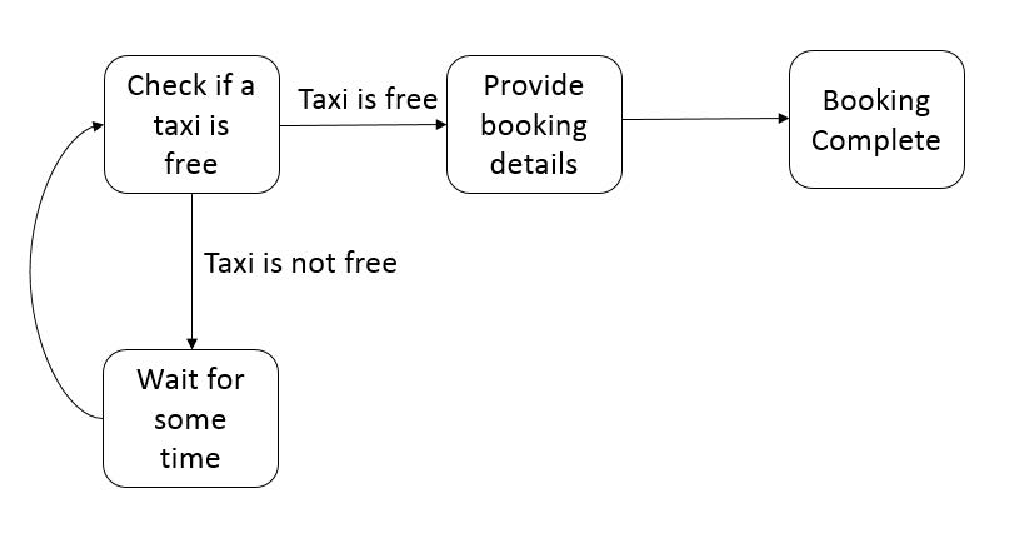
\includegraphics[scale = 0.5]{CPN_abstract_taxi_example.pdf}
	\caption{An abstract model for booking a taxi}
	\label{fig:CPN_abstract_taxi_example}
\end{figure}
\paragraph{\textnormal{Let us consider an example representing a simple online taxi booking service (see Figure \ref{fig:CPN_abstract_taxi_example}). To book a taxi the customer visits the web page. Upon visit, the booking service automatically generates a session identifier. To proceed with the booking process, the system checks for the available taxi. If the taxi is available, then the customer is asked to provide a phone number, pickup time and pickup address. Once the booking information is provided, the booking is finalised and the confirmation is shown to the user. If instead, no taxi is available, the user has to wait until a taxi is free.}}

\section{Coloured Petri Nets (CPNs) Syntax} \label{sec:CPN_Syntax}

\begin{figure}[!htbp]
	\centering
	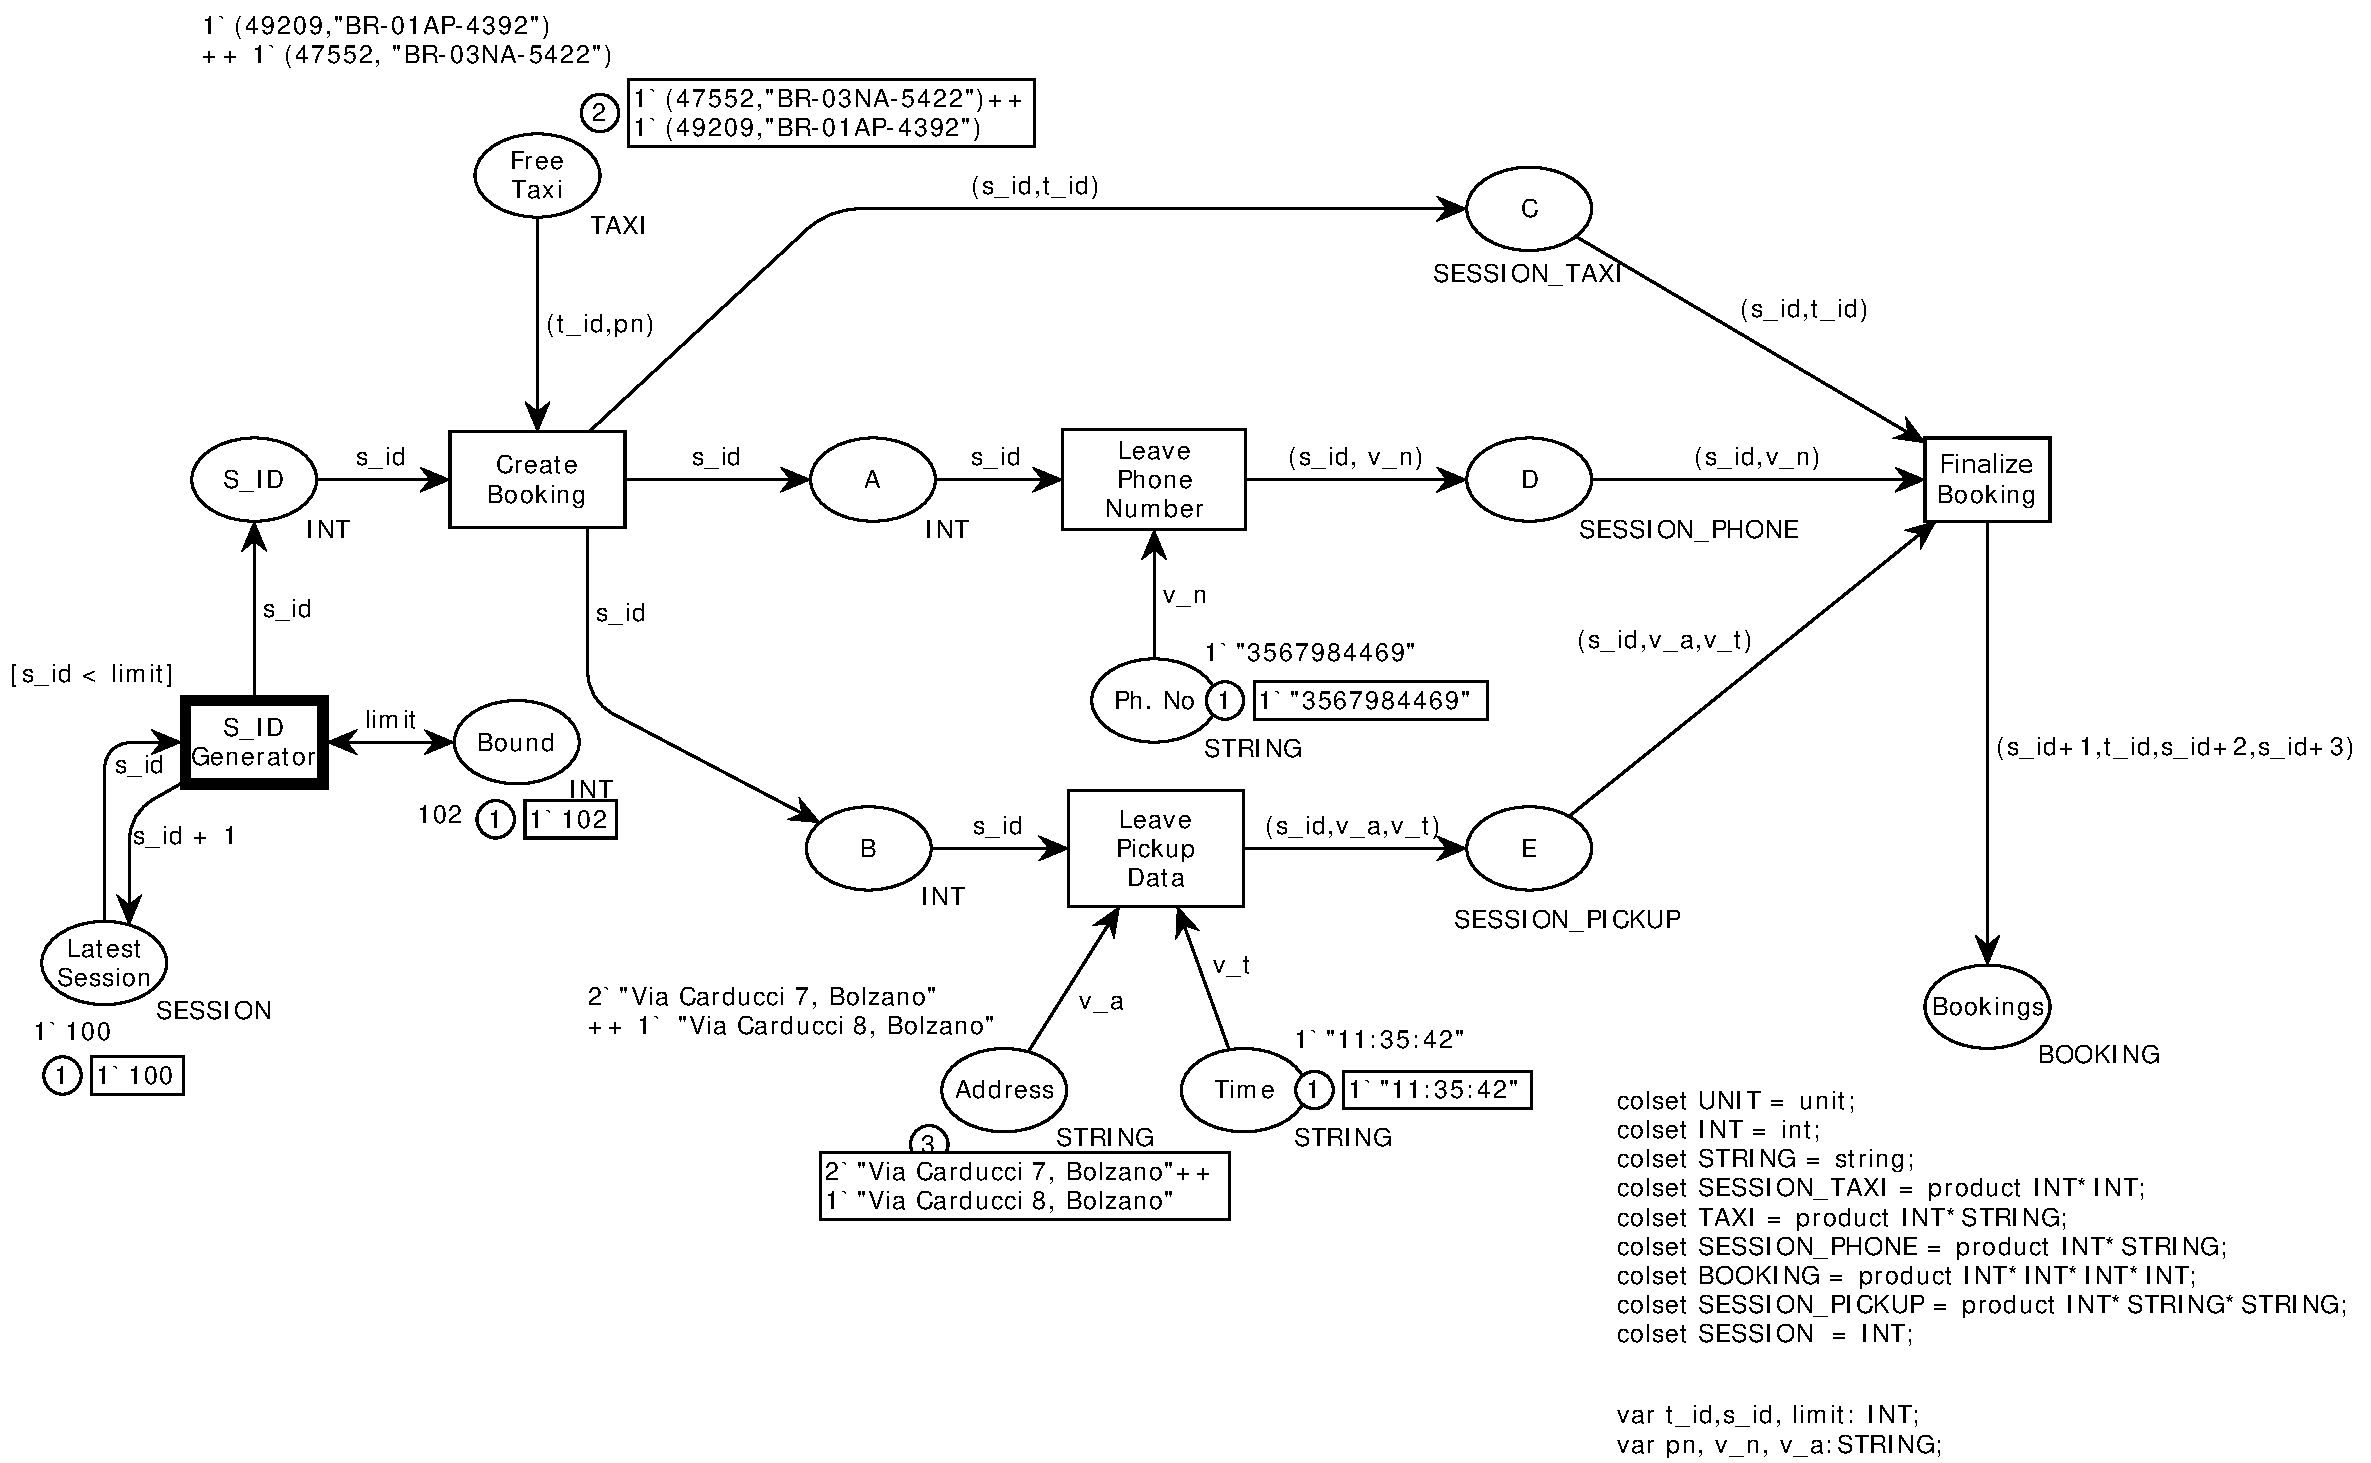
\includegraphics[scale = 0.35]{CPN_Taxi_Booking.pdf}
	\caption{CPN model for taxi booking}
	\label{fig:CPN_Taxi_Booking}
\end{figure}

\subparagraph*{\textnormal{Figure \ref{fig:CPN_Taxi_Booking} shows the CPN model\footnote{This example is modelled in a tool called \bdq{CPN Tools}\cite{CPN_Tools}. CPN Tools uses CPN ML as its programming language.} of the taxi booking example. Here, the places are represented by ellipses and the transitions are represented by rectangles. They are connected to each other by directed arcs. Places represent the state of the system. Each place contains tokens which have data value attached to it. This data value is called \textit{token colour} in CPN. Transitions represent events which can occur in the system. From the classical theory of Petri nets\cite{DBLP:books/daglib/Reisig2013} we know that Petri nets are directed bipartite graph and the bi-partition is between places and transitions, which means that places cannot be connected to places and transitions cannot be connected to transitions.}}

\subparagraph*{\textnormal{A session identifier is generated (at place $\mathit{Latest\ Session}$) incrementally with the starting value as 100. Only 2 session ids can be generated as the guard\footnote{A guard is a boolean expression attached to a transition. In order to make enable a transition, the corresponding guard must evaluate to $\mathit{True}$.} on the $\mathit{S\_ID}$ does not allow to have a session ID greater than the limit which is 102. The transition $\mathit{S\_ID\ Generator}$ is connected to the place $\mathit{Bound}$ with a double headed arc \footnote{It is counted as 2 arcs here, one connecting the place and the transition and the other connecting the same transition and place.}. It does not affect the content of the place. The process proceeds with checking the available taxi and providing the pickup details. $\mathit{Finalize\ Booking}$ transition is called and the confirmed booking is displayed at the place $\mathit{Booking}$. Each booking has a booking id, taxi id, phone id and pickup id. For simplicity and reduced the size of our CPN model, we abstract booking id, taxi id, phone id and pickup id in terms of $\mathit{s\_id}$. We represent them as:
\begin{equation*}
\begin{aligned}
booking\ id = & s\_id + 1\\
phone\ id = & s\_id + 2\\
pickup\ id = & s\_id + 3\\
\end{aligned}
\end{equation*}}}

\subparagraph*{\textnormal{The set of places, transitions, and arcs are denoted by $\mathit{P}$, $\mathit{T}$,and $\mathit{A}$ respectively. In Figure \ref{fig:CPN_Taxi_Booking}, there are 13 places, 5 transitions and 21 directed arcs. The set of places, transitions and arcs are :
\begin{equation*}
\begin{aligned}
P =\ & \{ S\_ID, Free\ Taxi, Address, Time, \ldots \}\footnotemark \\
T =\ &\{ Create\ Booking, Leave\ Phone\ Number, \ldots \} \\
A =\ & \{ (S\_ID, Create\ Booking), (Free\ Taxi, Create Booking),\ldots\}
\end{aligned}
\footnotetext{here in the set notation, \ldots means similarly there are other elements in the set, it should not be confused with an infinite set. The sets are finite.}
\end{equation*}}}

\subparagraph*{\textnormal{In Figure \ref{fig:CPN_Taxi_Booking}, the place $\mathit{Free\ Taxi}$ contains taxis which are not occupied, $\mathit{Bookings}$ contains all the bookings done so far. $\mathit{A}$, $\mathit{B}$, $\mathit{C}$, $\mathit{D}$, $\mathit{E}$ are intermediate places. Places $\mathit{Ph. No}$, $\mathit{Address}$ and $\mathit{Time}$ contain customer's phone number, pickup address and pickup time respectively. For a particular phone number, we have one phone ID which is contained in the place $\mathit{Phone\ ID}$. Similarly, for a booking we have booking id at the place $\mathit{Booking\ ID}$ and for the pickup data, we have a pickup id at place $\mathit{Pickup\ ID}$. The place $\mathit{S\_ID}$ corresponds to session id of a customer. A token is a pair of place and colour-set.}}

\subparagraph*{\textnormal{Each place has a data type attached to it, which is called \textbf{colour-set} of the place. In Figure \ref{fig:CPN_Taxi_Booking}, the colour-set of each place is defined at the bottom right of the place. For example, place $\mathit{S\_ID}$ has the colour-set INT, place $\mathit{Free\ Taxi}$ has the colour-set TAXI. The list of all the colour-set used is provided in Figure \ref{fig:CPN_Taxi_Booking} (in the bottom right corner). In CPN-ML\footnote{CPN Tools uses CPN-ML as its programming language. CPN-ML is an extension of standard ML. Standard ML is a functional programming language, in the sense that the full power of mathematical functions is present. A detailed description of SML is provided in \cite{milner1997definition}. In order to get acquainted with ML programming language in brief and how it used as a programming language with CPN, one can read \cite{Jensen_CPN_Book_ML}.}, the colour-set is written by prefixing the keyword \bdq{COLSET}. The colour-sets STRING and INT are defined as the primitive data type \bdq{string} and \bdq{int} respectively. The colour-set TAXI contains pair (INT, STRING), where the first element represents the taxi id and the second element represents the corresponding plate number.  Similarly, other colour-sets are defined. In general, a colour-set can be cartesian product of different data types.}}

\subparagraph*{\textnormal{We can also restrict the values that a particular colour-set can take. This makes the domain of the colour-set finite\footnote{More information on making finite colour-set is given in \cite{CPN_Tools_ColourSet}}. This is achieved by using the \bdq{with} clause while declaring the colour-set. One such code is provided below. In this code, when we declare the colour-set \bsq{SESSION} we put a limit on the colour-set stating that the value of the integer cannot be less than 100 or greater than 102. Hence by limiting the domain of the colour-set \bsq{SESSION} in the interval $\mathit{\left[100,102\right]}$, we restrict the model to generate a maximum of 2 session ids.}}

\begin{verbatim}
COLSET SESSION = int with 100..102;
\end{verbatim}

\subparagraph*{\textnormal{A \textit{marking} represents the state of the CPN model which is determined by the number of tokens and the token colours on individual places. The marking of a place is determined by the tokens on the specific place. We use the multiset $\mathit{m_{Address}}$ and $\mathit{m_{Free Taxi}}$ to denote the multiset over the colour-set STRING and TAXI respectively corresponding to the markings of the places $\mathit{Address}$ and $\mathit{Free\ Taxi}$ in Figure \ref{fig:CPN_Taxi_Booking}:
\begin{equation*}
\begin{aligned}
&m_{Address} = {2}^{\backprime}\textnormal{"Via Carducci 7, Bolzano"} +\!\!+\ {1}^{\backprime}\textnormal{"Via Carducci 8, Bolzano"}\\
&m_{Free Taxi} = {1}^{\backprime}\textnormal{(49209,\bdsq{(BR-01AP-4392)}} +\!\!+\ {1}^{\backprime}\textnormal{(47552, \bdsq{BR-03NA-5422})}
\end{aligned}
\end{equation*}
This indicates that the place \textit{Address} has the marking which contains 2 tokens of data value \bdsq{Via Carducci 7, Bolzano} and 1 token of data value \bdsq{Via Carducci 8, Bolzano}. The reason for these data values are written in double quotes is because they are of type string. If the number of tokens is 1 then we can omit the number and the ${}^{\backprime}$ operator, and simply write the data value. e.g. ${1}^{\backprime}$\bdsq{Via Carducci 8, Bolzano} can be simply written as \bdsq{Via Carducci 8, Bolzano}. The multiset $m_{Address}$ can be defined as:
\begin{equation*}
m_{Address}(s) = \begin{cases}
2 & \textit{if s = \textnormal{\bdsq{Via Carducci 7, Bolzano}}} \\ 
1 & \textit{if s = \textnormal{\bdsq{Via Carducci 8, Bolzano}}} \\ 
0 & \textit{otherwise}
\end{cases}
\end{equation*}
Similarly, for the place $\mathit{Free\ Taxi}$, one could write it as:
\begin{equation*}
m_{Free Taxi}(s) = \begin{cases}
1 & \textit{if s = \textnormal{(49209,\bdsq{BR-01AP-4392})}} \\ 
1 & \textit{if s = \textnormal{(47552,\bdsq{BR-03NA-5422})}} \\ 
0 & \textit{otherwise} 
\end{cases}
\end{equation*}}}
\begin{comment}
Where the ${}^{\backprime}$ is the infix operator, the number preceding the symbol ${}^{\backprime}$ signifies the number of tokens while the tuple succeeding the symbol represents the data value.	content...
\end{comment}

\subparagraph*{\textnormal{Let us now formally define elements that constitute \textbf{net inscriptions}, i.e., arc expressions, guards and colour-sets. Arc expressions are the expressions written on the arcs. We denote by $\mathit{EXPR}$ the set of expressions provided by the inscription language. Here, the inscription language is a general term for a backend language used to specify colour-sets and operations over them. However, in our case, we rely on a specific language, i.e., CPN ML provided by CPNTools. Given an expression $\mathit{e \in EXPR}$, the \textbf{\textit{type}} of $\mathit{e}$, represented by $\mathit{Type[e]}$, specifies the colour of values obtained by evaluating $\mathit{e}$. The set of \textbf{\textit{free variables}} in an expression $\mathit{e}$ is denoted by $\mathit{Var[e]}$, and the type of a variable $\mathit{v}$ is denoted by $\mathit{Type[v]}$. $\mathit{V}$ denotes the set of variables. Note that a free variable is a variable which is not bound in the local environment of the expression.
In Figure \ref{fig:CPN_Taxi_Booking}, for the arc expressions we have the following free variables:
\begin{equation*}
\mathit{Var[e]} = \begin{cases}
\mathit{\{s\_id\}} & \textit{if e = s\_id}\\ 
\mathit{\{t\_id, pn\}} & \textit{if e = \textnormal{(}t\_id, pn\textnormal{)}} \\ 
\mathit{\{s\_id, t\_id\}} & \textit{if e = \textnormal{(}s\_id, t\_id\textnormal{)}} \\ 
\mathit{\{v\_n\}} & \textit{if e = \textnormal{(}v\_n\textnormal{)}}\\ 
\ldots
\end{cases}
\end{equation*}}}
\subparagraph*{\textnormal{$\mathit{\Sigma}$ denotes the set of \textbf{\textit{colour-sets}} defined for the CPN model. Given a set of variables $\mathit{V}$, for all $\mathit{v \in V : Type[v] \in \Sigma}$. For $\mathit{V' \subseteq V}$, the set of expressions $\mathit{e \in EXPR}$ such that $\mathit{Var[e] \subseteq V'}$ is denoted $\mathit{EXPR_{V'}}$. For the CPN model in Figure \ref{fig:CPN_Taxi_Booking}, the colour-sets are defined as:
\begin{equation*}
\begin{aligned}
\mathit{\Sigma = \{ INT, STRING, TAXI, SESSION\_TAXI, \ldots \}}
\end{aligned}
\end{equation*}
We define the set of free variables in our CPN model:
\begin{equation*}
\begin{aligned}
\mathit{V = \{s\_id : INT, t\_id : INT, v\_a : STRING, v\_t : STRING, \ldots\}}
\end{aligned}
\end{equation*}}}

\subparagraph*{\textnormal{The \textbf{\textit{colour-set function}} is a function, $\mathit{C : P \rightarrow \Sigma}$, which maps every place to its corresponding colour-set. The colour-set function for the CPN model in Figure \ref{fig:CPN_Taxi_Booking} is:}}

\begin{equation*}
C(p) = \begin{cases}
\mathit{INT} & \textit{if p $\in$ \textnormal{\{}S\_ID, A, B, Bound\textnormal{\}}}\\
\mathit{STRING} & \textit{if p $\in$ \textnormal{\{}Ph. No, Address, Time\textnormal{\}}}\\
\mathit{TAXI} & \textit{if p = Free Taxi}\\
\mathit{SESSION\_TAXI} & \textit{if p = C}\\
\mathit{SESSION\_PHONE} & \textit{if p = D}\\
\mathit{SESSION\_PICKUP} & \textit{if p = E}\\
\mathit{BOOKING} & \textit{if p = Bookings} \\
\mathit{SESSION} & \textit{if p = Latest Session}
\end{cases}
\end{equation*}
\paragraph*{\textnormal{\textit{Guard} is a boolean expression attached to the transitions. For a transition be enabled it is a necessary condition that the guard of the transition should evaluate to $\mathit{True}$. A function $\mathit{G : T \rightarrow EXPR_{V}}$ is called a \textbf{\textit{guard function}} and assigns every transition $\mathit{t \in T}$ a boolean expression, i.e., $\mathit{Type[G(t)] = Bool}$. The set of free variables occurring in a guard should be a subset of $\mathit{V}$, hence, $\mathit{G(t) \in EXPR_{V}}$. The CPN model, in Figure \ref{fig:CPN_Taxi_Booking}, has guard function defined as:
}}

\begin{equation*}
G(t) = \begin{cases}
\mathit{s\_id < limit} & $\textit{if t = S\_ID Generator}$\\
\mathit{True} & $\textit{otherwise}$
\end{cases}
\end{equation*}

\subparagraph*{\textnormal{A function $E : A \rightarrow EXPR_{V}$ is called \textbf{\textit{arc expression function}} which assigns every $a \in A$ an expression $E(a)$. Similar to the guards of the transition, the free variables occurring in $E(a)$ has to be a subset of $V$, hence, $E(a) \in EXPR_{V}$. For an arc $(p,t) \in A$, connecting a place $p \in P$ and a transition $t \in T$, it is required that the type of the arc expression is the multiset type over the colour-set $C(p)$ of the place $p$, i.e., $Type[E(p, t)] = C(p)_{MS}$. This is for the directed arc from a place to a transition. Similarly it can be applied to a directed arc from a transition to a place. For an arc $(t,p) \in A$ it is required that $Type[E(t, p)] = C(p)_{MS}$. For the model in Figure \ref{fig:CPN_Taxi_Booking}, the arc expression function is defined as:}}
\begin{equation*}
E(a) = \begin{cases}
{1}^{\backprime}(s\_id) & \textit{if a $\in$ \textnormal{\{(}S\_ID, Create Booking\textnormal{)},}\\
& \textit{\textnormal{(}Create Booking, A\textnormal{)},\textnormal{(}Create Booking, B\textnormal{)},}\\
& \textit{\textnormal{(}A, Leave Phone Number\textnormal{)},}\\ 
& \textit{\textnormal{(}B, Leave Pickup Data\textnormal{)\}}}\\
{1}^{\backprime}(s\_id,t\_id) & \textit{if a $\in$ \textnormal{\{(}Create Booking, C\textnormal{)},}\\ 
& \textit{\textnormal{(}E, Finalize Booking\textnormal{)\}}}\\
{1}^{\backprime}(v\_n) & \textit{if a = \textnormal{(}Ph. No, Leave Phone Number\textnormal{)}}\\
\ldots
\end{cases}
\end{equation*}

\subparagraph*{\textnormal{The initialization function gives initial marking to all places in the model. The \textbf{\textit{initialization function}} $\mathit{I : P \rightarrow EXPR_{0}}$ assigns to each place $\mathit{p}$ an initialization expression $\mathit{I(p)}$ which is required to evaluate to a multiset over the colour-set of the place $\mathit{p}$, i.e., $\mathit{Type[I(p)] = C(p)_{MS}}$. The initialization expression must be a closed expression, i.e., it cannot have any free variables, hence $\mathit{I(p) \in EXPR_{\emptyset}}$. A possible initialization function for the model in Figure \ref{fig:CPN_Taxi_Booking} is given by:
\begin{equation*}
I(p) = \begin{cases}
\textnormal{${1}^{\backprime}$(49209,\bdsq{BR-01AP-4392})} +\!\!+  & \textit{if p = Free Taxi}\\
\textnormal{${1}^{\backprime}$(47552,\bdsq{BR-03NA-5422})} & \\
\textnormal{${2}^{\backprime}$\bdsq{Via Carducci 7, Bolzano}} +\!\!+ & \textit{if p = Address}\\ 
\textnormal{${1}^{\backprime}$\bdsq{Via Carducci 8, Bolzano}} & \\
\textnormal{${1}^{\backprime}$\bdsq{11:35:42}} & \textit{if p = Time}\\
\textnormal{${1}^{\backprime}$\bdsq{3567984469}} & \textit{if p = Ph. No}\\
\textnormal{${1}^{\backprime}$100} & \textit{if p = Latest Session}\\
\textnormal{${1}^{\backprime}$102} & \textit{if p = Bound}\\
\emptyset_{MS} & \textit{otherwise}
\end{cases}
\end{equation*}}}

\subparagraph*{\textnormal{With the explanation of the above functions, we  define non-hierarchical coloured petri nets.}}

\begin{defs}
	\label{defs:CPN_NonHeir}
	A non-hierarchical Coloured Petri Net is a tuple $\mathit{CPN} = \mathit{(P,T,A,\Sigma,V,C,G,E,I)}$, where:
	\begin{itemize}
		\item $\mathit{P}$ is a finite set of places.
		\item $\mathit{T}$ is a finite set of transitions $\mathit{T}$ such that $\mathit{P \cap T = \emptyset}$.
		\item $\mathit{A \subseteq (P \times T) \cup (T \times P)}$ is a set of directed arcs.
		\item $\mathit{\Sigma}$ is a finite set of non-empty colour-sets.
		\item $\mathit{V}$ is a finite set of typed variables such that $\mathit{Type[v] \in \Sigma}$ for all variables $\mathit{v \in V}$.
		\item $\mathit{C : P \rightarrow \Sigma}$ is a colour-set function that assigns a colour-set to each place.
		\item $\mathit{G : T \rightarrow EXPR_{V}}$ is a guard function that assigns a guard to each transition $\mathit{t}$ such that $\mathit{Type[G(t)] = Bool}$.
		\item $\mathit{E : A \rightarrow EXPR_{V}}$ is an arc expression function that assigns an arc expression to each arc $\mathit{a}$ such that $\mathit{Type[E(a)] = C(p)_{MS}}$, where $\mathit{p}$ is the place connected to the arc $\mathit{a}$.
		\item $\mathit{I : P \rightarrow EXPR_{\emptyset}}$ is an initialization function that assigns an initialization expression to each place $\mathit{p}$ such that $\mathit{Type[I(p)] =C(p)_{MS}}$.
	\end{itemize}
\end{defs}

\section{Colored Petri Nets (CPNs) Semantics} \label{sec:CPN_Semantics}
\paragraph{\textnormal{In this section, we discuss about markings and binding elements. Later, we look at a step, enabling and occurrence of steps and when a step occurs how it effects the marking of the net. We also discuss the conditions when the transition is enabled. In the end, we discuss reachable markings and state spaces.}}
\subsection*{Enabling and Occurrence of Steps}

\begin{comment}
\paragraph{\textnormal{In this section, we discuss about markings and binding elements. Later, we look at a step, enabling and occurrence of steps and when a step occurs how it effects the marking of the net. We also discuss the conditions when the transition is enabled. In the end, we discuss reachable markings and state spaces.}}
\end{comment}

\subparagraph{\textnormal{In a given marking, the enabling rule specifies when a step (consisting of a multiset of binding elements) becomes enabled, whereas the firing/occurrence rule specifies how the markings change when the enabled step occurs.}}

\begin{figure}[!htbp]
	\centering
	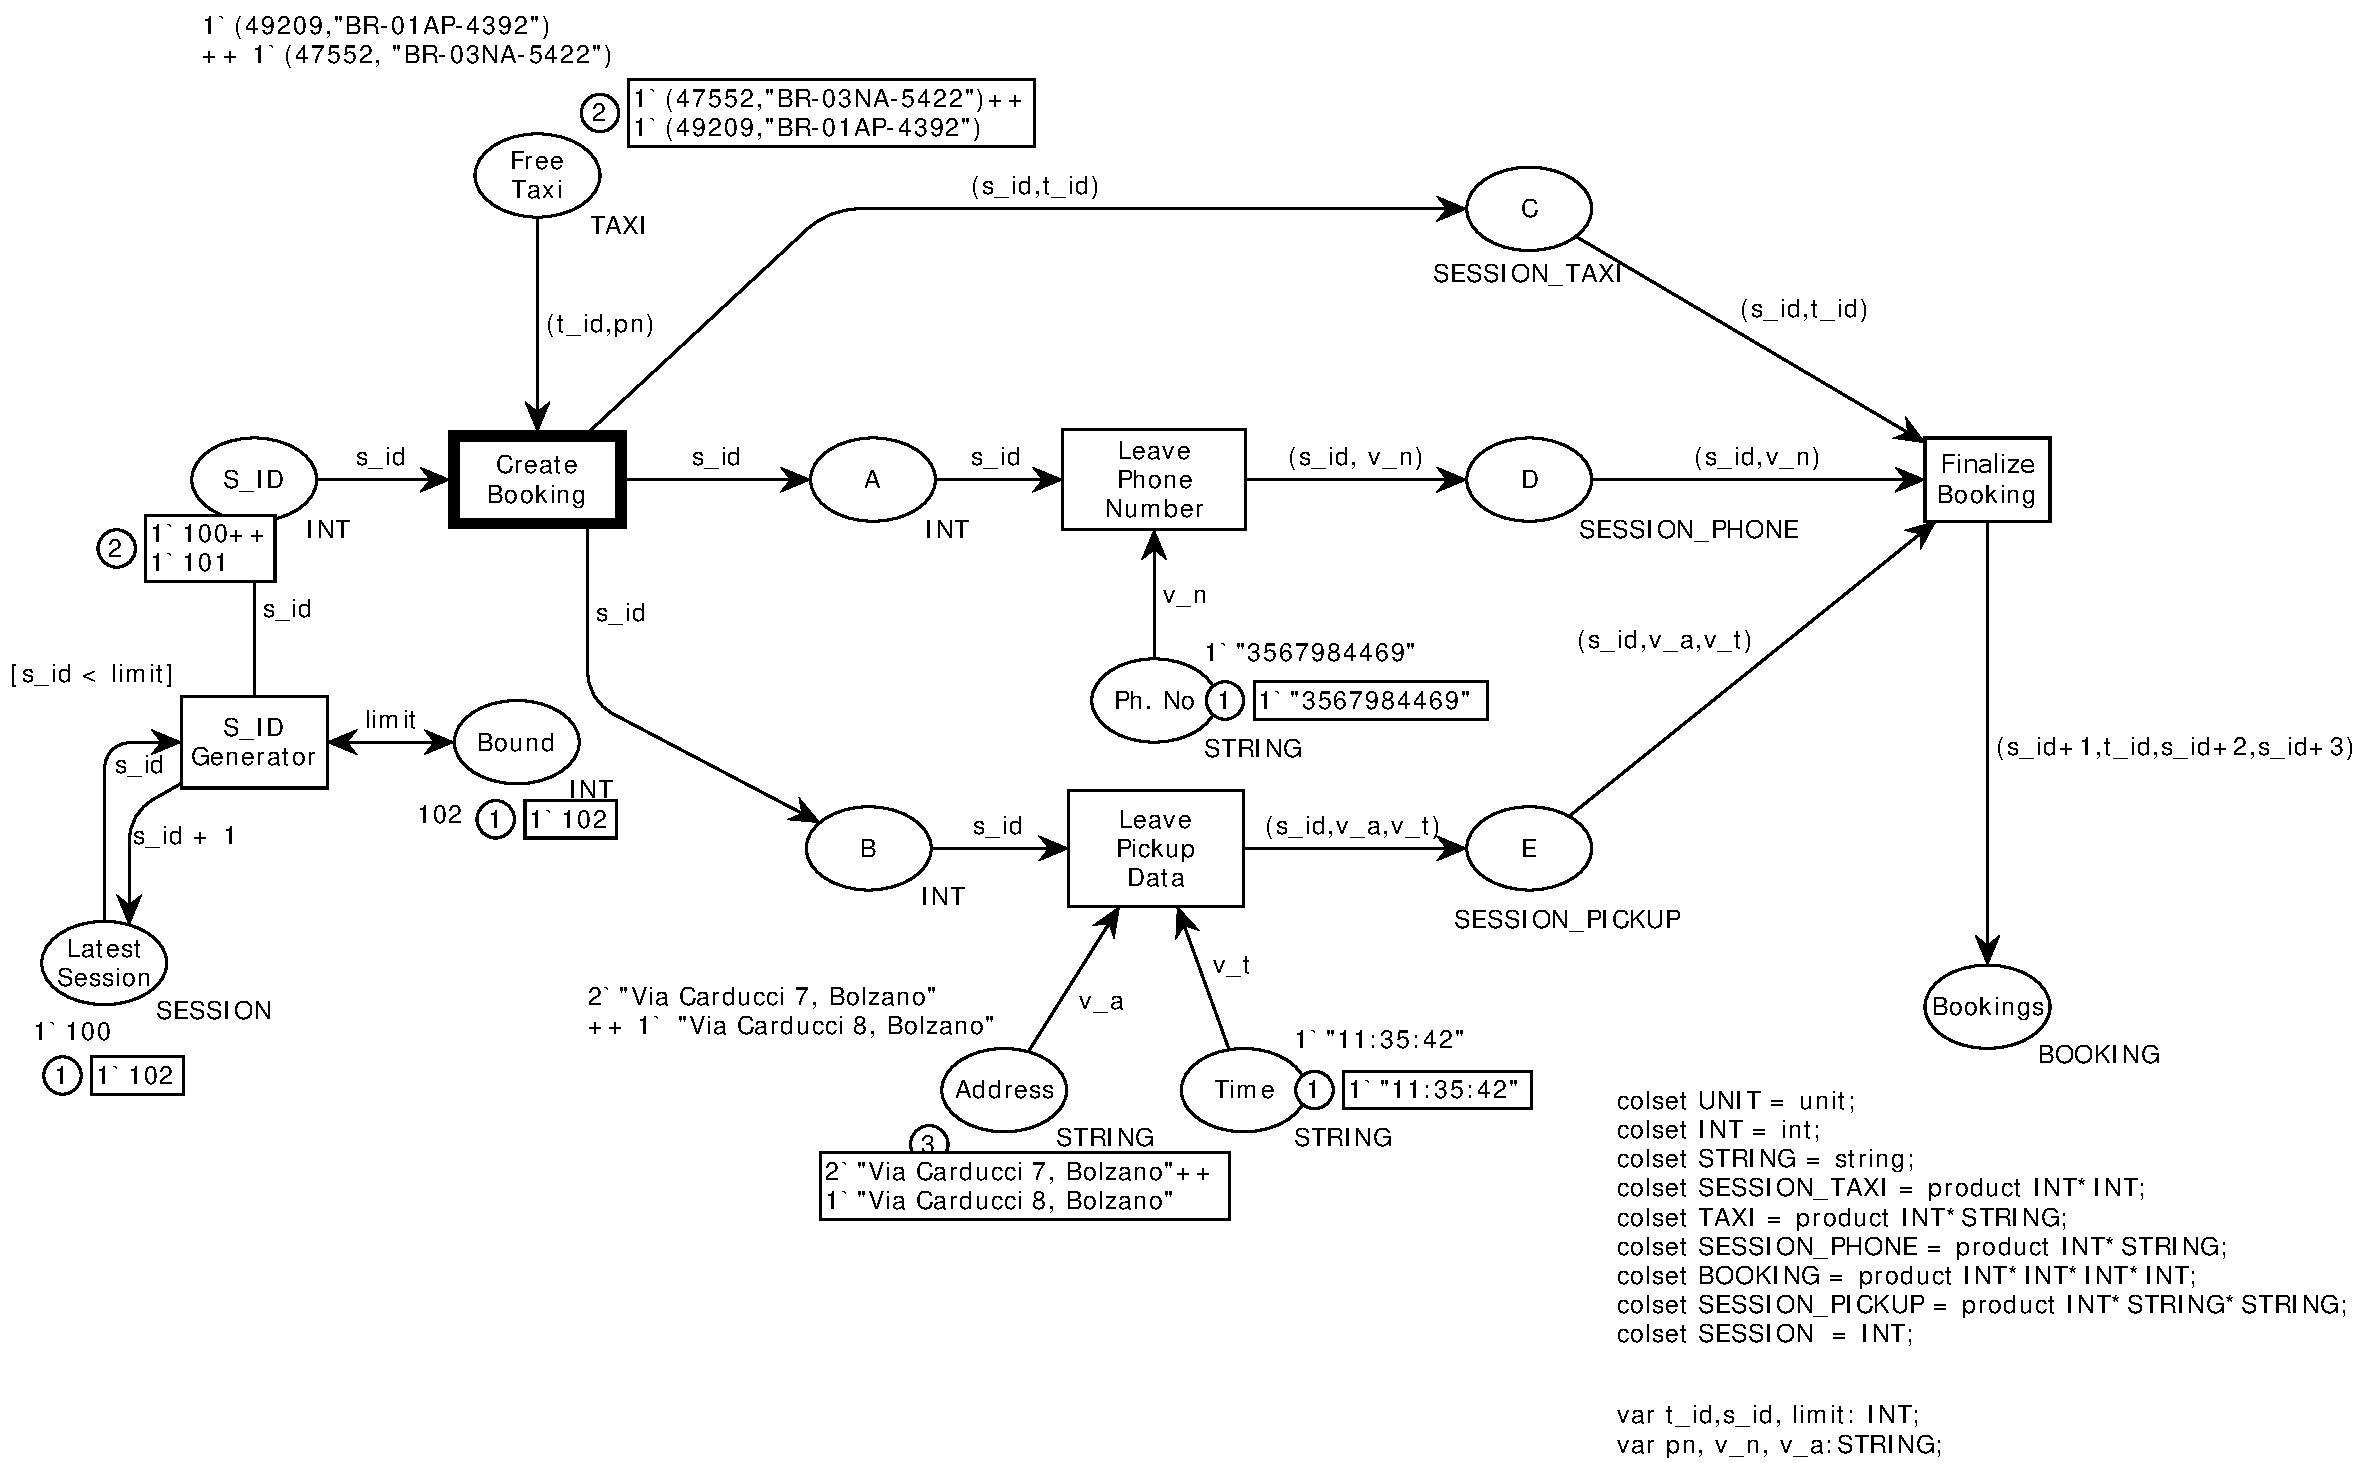
\includegraphics[scale = 0.35]{CPN_Taxi_Booking_initial_step.pdf}
	\caption{CPN model for taxi booking}
	\label{fig:CPN_Taxi_Booking_initial_step}
\end{figure}

\subparagraph*{\textnormal{A \textbf{\textit{marking}} $\mathit{M}$ is a function that maps each place $\mathit{p}$ into a multiset of values $\mathit{M(p)}$ representing the marking of $\mathit{p}$. The individual elements in the multiset $\mathit{M(p)}$ are called \textbf{\textit{tokens}}. The multiset of tokens present on a place $\mathit{p}$ in a marking $\mathit{M}$ is required to match the type of the place, i.e., $\mathit{M(p) \in C(p)_{MS}}$. For example, the marking of the places for the CPN model presented in Figure \ref{fig:CPN_Taxi_Booking_initial_step} is given by\footnote{The markings in the model are represented by rectangles beside each place.}:}}

\begin{equation*}
M(p) = \begin{cases}
{1}^{\backprime}100 +\!\!+ {1}^{\backprime}101 & \textit{if p = S\_ID}\\
\textnormal{${1}^{\backprime}$(49209,\bdsq{BR-01AP-4392})} +\!\!+  & \textit{if p = Free Taxi}\\
\textnormal{${1}^{\backprime}$(47552,\bdsq{BR-03NA-5422})} & \\
\textnormal{${2}^{\backprime}$\bdsq{Via Carducci 7, Bolzano}} +\!\!+ & \textit{if p = Address}\\ 
\textnormal{${1}^{\backprime}$\bdsq{Via Carducci 8, Bolzano}} & \\
\textnormal{${1}^{\backprime}$\bdsq{11:35:42}} & \textit{if p = Time}\\
\textnormal{${1}^{\backprime}$\bdsq{3567984469}} & \textit{if p = Ph. No}\\
\textnormal{${1}^{\backprime}$102} & \textit{if p = Latest Session}\\
\textnormal{${1}^{\backprime}$102} & \textit{if p = Bound}\\
\emptyset_{MS} & \textit{otherwise}
\end{cases}
\end{equation*}

\subparagraph*{\textnormal{$\mathit{Var(t)}$ denotes \textbf{\textit{variables of a transition}} $\mathit{t}$, which consists of free variables appearing either in any of the arc expression connecting the transition or in the guard of the transition. The variables for the transitions for the model in the Figure \ref{fig:CPN_Taxi_Booking_initial_step} are:}}
\begin{equation*}
Var(t) = \begin{cases}
\{s\_id,t\_id,pn\} & \textit{if t = Create Booking}\\
\{s\_id,v\_n\} & \textit{if t = Leave Phone Number}\\
\{s\_id,v\_a,v\_t\} & \textit{if t = Leave Pickup Data}\\
\{s\_id,t\_id,v\_n,v\_a,v\_t\} & \textit{if t = Finalize Booking}\\
\{s\_id,limit\} & \textit{if t = S\_ID Generator} 
\end{cases}
\end{equation*}

\subparagraph*{\textnormal{The \textbf{\textit{initial marking}}, denoted by $\mathit{M_{0}}$, is obtained by evaluating the initialization expression. The initialization expression does not contain any free variables and its evaluation is with the empty binding (denoted by $\mathit{\langle \rangle}$), i.e., $\mathit{M_{0}(p) = I(p)\langle \rangle,}$ for each $\mathit{p \in P}$. The initial marking for this example (Figure \ref{fig:CPN_Taxi_Booking}) is given by:}}

\begin{equation*}
M_{0}(p) = \begin{cases}
\textnormal{${1}^{\backprime}$(49209,\bdsq{BR-01AP-4392})} +\!\!+  & \textit{if p = Free Taxi}\\
\textnormal{${1}^{\backprime}$(47552,\bdsq{BR-03NA-5422})} & \\
\textnormal{${2}^{\backprime}$\bdsq{Via Carducci 7, Bolzano}} +\!\!+ & \textit{if p = Address}\\ 
\textnormal{${1}^{\backprime}$\bdsq{Via Carducci 8, Bolzano}} & \\
\textnormal{${1}^{\backprime}$\bdsq{11:35:42}} & \textit{if p = Time}\\
\textnormal{${1}^{\backprime}$\bdsq{3567984469}} & \textit{if p = Ph. No}\\
\textnormal{${1}^{\backprime}$100} & \textit{if p = Latest Session}\\
\textnormal{${1}^{\backprime}$102} & \textit{if p = Bound}\\
\emptyset_{MS} & \textit{otherwise}
\end{cases}
\end{equation*}

\subparagraph*{\textnormal{A \textbf{\textit{binding}} $b$ of a transition $t$ is a function that maps each variable $v$ of the transition $t$ to a value $b(v)$ belonging to the type of the variable $v$, i.e., $b(v) \in Type[v]$. Bindings are written as $\langle var_{1} = val_{1},var_{2} = val_{2}, \ldots ,var_{n} = val_{n} \rangle$, where $var_{1}, var_{2}, \ldots , var_{n}$ are the variables in $Var(t)$ and $val_{i}$ is the value bound to the variable $var_{i}$. A \textbf{\textit{binding element}} is a pair $(t,b)$ consisting of a transition $t$ and a binding $b$ of $t$. A step is a non-empty, finite multiset of binding elements.}}

\subparagraph*{\textnormal{With the above functions at hand, we define few concepts related to CPN.}}

\begin{defs}
	\label{defs:2_7_step_marking}
	For a Coloured Petri Net $\mathit{CPN = (P,T,A,\Sigma,V,C,G,E,I)}$:
	\begin{enumerate}
		\item A \textbf{marking} is a function $\mathit{M}$ that maps each place $\mathit{p \in P}$ into a multiset of tokens
		$\mathit{M(p) \in C(p)_{MS}}$.
		\item The \textbf{initial marking} $\mathit{M_{0}}$ is defined by $\mathit{M_{0}(p) = I(p)}$ for all $\mathit{p \in P}$.
		\item The \textbf{variables of a transition} $\mathit{t}$ are denoted $\mathit{Var(t) \subseteq V}$ and consist of the free variables appearing in the guard of $\mathit{t}$ and in the arc expressions of arcs connected to $\mathit{t}$.
		\item A \textbf{binding} of a transition $\mathit{t}$ is a function $\mathit{b}$ that maps each variable $\mathit{v \in Var(t)}$ into a value $\mathit{b(v) \in Type[v]}$. The set of all bindings for a transition $\mathit{t}$ is denoted $\mathit{B(t)}$.
		\item A \textbf{binding element} is a pair $\mathit{(t,b)}$ such that $\mathit{t \in T}$ and $\mathit{b \in B(t)}$. The set of all binding elements $\mathit{BE(t)}$ for a transition $\mathit{t}$ is defined by $\mathit{BE(t)} = \mathit{\{(t,b) | b \in B(t)\}}$. The set of all binding elements in a CPN model is denoted $\mathit{BE}$.
		\item A \textbf{step} $\mathit{Y \in BE_{MS}}$ is a non-empty, finite multiset of binding elements.
	\end{enumerate}
\end{defs}

\subparagraph*{\textnormal{As stated earlier, the transitions have guards attached to them and the arcs carry expressions with them (arc expressions). These two determine the enabling and occurrence of a step. For a binding element $\mathit{(t,b)}$ where $\mathit{t}$ is a transition and $\mathit{b}$ is a binding, the guard expression $\mathit{G(t)}$ of the transition is evaluated against the binding $\mathit{b}$ and the result is written as $\mathit{G(t)\langle b \rangle}$. Similarly, the arc expression $\mathit{E(a)}$ (for any arc $\mathit{a}$) is also evaluated against the binding $\mathit{b}$ and the result is written as $\mathit{E(a)\langle b \rangle}$. For an arc $\mathit{a = (p,t)}$, which connects a place $\mathit{p}$ and a transition $\mathit{t}$, the arc expression $\mathit{E(p,t)}$ denotes the arc expression on the input arc from $\mathit{p}$ to $\mathit{t}$. When no such arc exists, we define $\mathit{E(p, t) = \emptyset_{MS}}$. Analogously, $\mathit{E(t, p)}$ denotes the arc expression on the output arc from $\mathit{t}$ to $\mathit{p}$. When no such arc exists, we define $\mathit{E(t, p) = \emptyset_{MS}}$.}}

\subparagraph*{\textnormal{For a binding $\mathit{(t,b)}$ to be enabled in a making $M$ there are two conditions to satisfy:
\begin{itemize}
\item The evaluation of the guard expression - In order for a binding to get enabled, the corresponding guard expression must evaluate to $\mathit{True}$.
\item The number of tokens in the input place - for each place $\mathit{p}$, an arc expression $\mathit{E(p,t)}$ has to be evaluated to the binding $\mathit{b}$ such that $\mathit{E(p,t)\langle b \rangle\ll=M(P)}$. It means that for each place $\mathit{p}$ there should be enough tokens that transition $\mathit{t}$ will remove when occurring with binding $\mathit{b}$.
\end{itemize}
}}

\subparagraph*{\textnormal{Let us look at the two conditions in our taxi booking example. Since we do not have any guards on our model the guard function evaluates to $\mathit{True}$ for all transitions in the model. Let us consider a binding element $\mathit{(Create\ Booking, b_{CB})}$ where
\begin{equation}
\label{eq:binding_1}
b_{CB} = \langle s_{id} = 100, t_{id} = 47552, pn = \textnormal{"BR-03NA-5422"}\rangle
\end{equation}
Alternatively, $b_{CB}$ can also be chosen as:
\begin{equation}
\label{eq:binding_2}
b_{CB} = \langle s_{id} = 101, t_{id} = 49209, pn = \textnormal{"BR-01AP-4392"}\rangle
\end{equation}
One of the important properties of CPN is non-determinism. Here, the values for the binding $\mathit{b_{CB}}$ can be chosen non-deterministically. Here, we will select the binding given in equation \ref{eq:binding_1}. From the input arcs of the $\mathit{Create\ Booking}$ transition, we have
\begin{equation*}
\begin{aligned}
E(S\_ID, Create\ Booking)\langle b_{CB}\rangle =& {1}^{\backprime}100 \ll = {1}^{\backprime}100\ +\!\!+\ {1}^{\backprime}101\\
E(Free\ Taxi, Create\ Booking)\langle b_{CB}\rangle =& {1}^{\backprime}(47552,\textnormal{"BR-03NA-5422"})\\ 
& \ll = {1}^{\backprime}(49209,\textnormal{"BR-01AP-4392"}) +\!\!+\ \\
& {1}^{\backprime}(47552,\textnormal{"BR-03NA-5422"})
\end{aligned}
\end{equation*}}}

\subparagraph*{\textnormal{When an enabled binding $\mathit{(t,b)}$ occurs \footnote{The thick border around the transition (see Figure \ref{fig:CPN_Taxi_Booking_initial_step}) signifies that the transition is enabled.}, the tokens are consumed from the input place and produced at the output place. The amount of tokens consumed or produced depends on the arc inscription attached to the respective arcs. The multiset of tokens removed from the input place $\mathit{p}$, when $\mathit{t}$ occurs in $\mathit{b}$ is given by $\mathit{E(p,t)\langle b \rangle}$, and the multiset of tokens added to an output place $\mathit{p}$ is given by: $\mathit{E(t,p)\langle b \rangle}$, which means that the new marking $\mathit{M'}$ reached when an enabled binding element $\mathit{(t,b)}$ occurs in a marking $\mathit{M}$ is given by:
\begin{equation*}
M'(p) = (M(p) -\!-\ E(p, t)\langle b \rangle) +\!\!+\ E(t, p)\langle b \rangle , \forall p \in P
\end{equation*}}}

\subparagraph*{\textnormal{For our model in Figure \ref{fig:CPN_Taxi_Booking}, let us calculate the new marking $M^{'}$ assuming the binding element (\textit{Create Booking, $b_{CB}$}) occurs.}}
\begin{equation*}
\begin{aligned}
M^{'}(S\_ID) =\ & ({1}^{\backprime}100\ +\!\!+\ {1}^{\backprime}101 -\!- \ {1}^{\backprime}100) +\!\!+\ \emptyset_{MS}\\
=\ & {1}^{\backprime}101 \\
M^{'}(Free\ Taxi) =\ & ({1}^{\backprime}(49209,\textnormal{"BR-01AP-4392"}) +\!\!+\ {1}^{\backprime}(47552,\textnormal{"BR-03NA-5422"})\\  
& -\!-\ {1}^{\backprime}(47552,\textnormal{"BR-03NA-5422"})) +\!\!+\ \emptyset_{MS}\\ 
=\ & {1}^{\backprime}(49209,\textnormal{"BR-01AP-4392"})\\ 
M^{'}(A) =\ &(\emptyset_{MS} -\!-\ \emptyset_{MS}) +\!\!+\ {1}^{\backprime}100 \\
=\ &{1}^{\backprime}100\\
M^{'}(B) =\ &(\emptyset_{MS} -\!-\ \emptyset_{MS}) +\!\!+\ {1}^{\backprime}100 \\
=\ &{1}^{\backprime}100\\
M^{'}(C) =\ &(\emptyset_{MS} -\!-\ \emptyset_{MS}) +\!\!+\ {1}^{\backprime}(100,47552)\\
=\ &{1}^{\backprime}(100,47552)
\end{aligned}
\end{equation*}

\begin{figure}[!htbp]
	\centering
	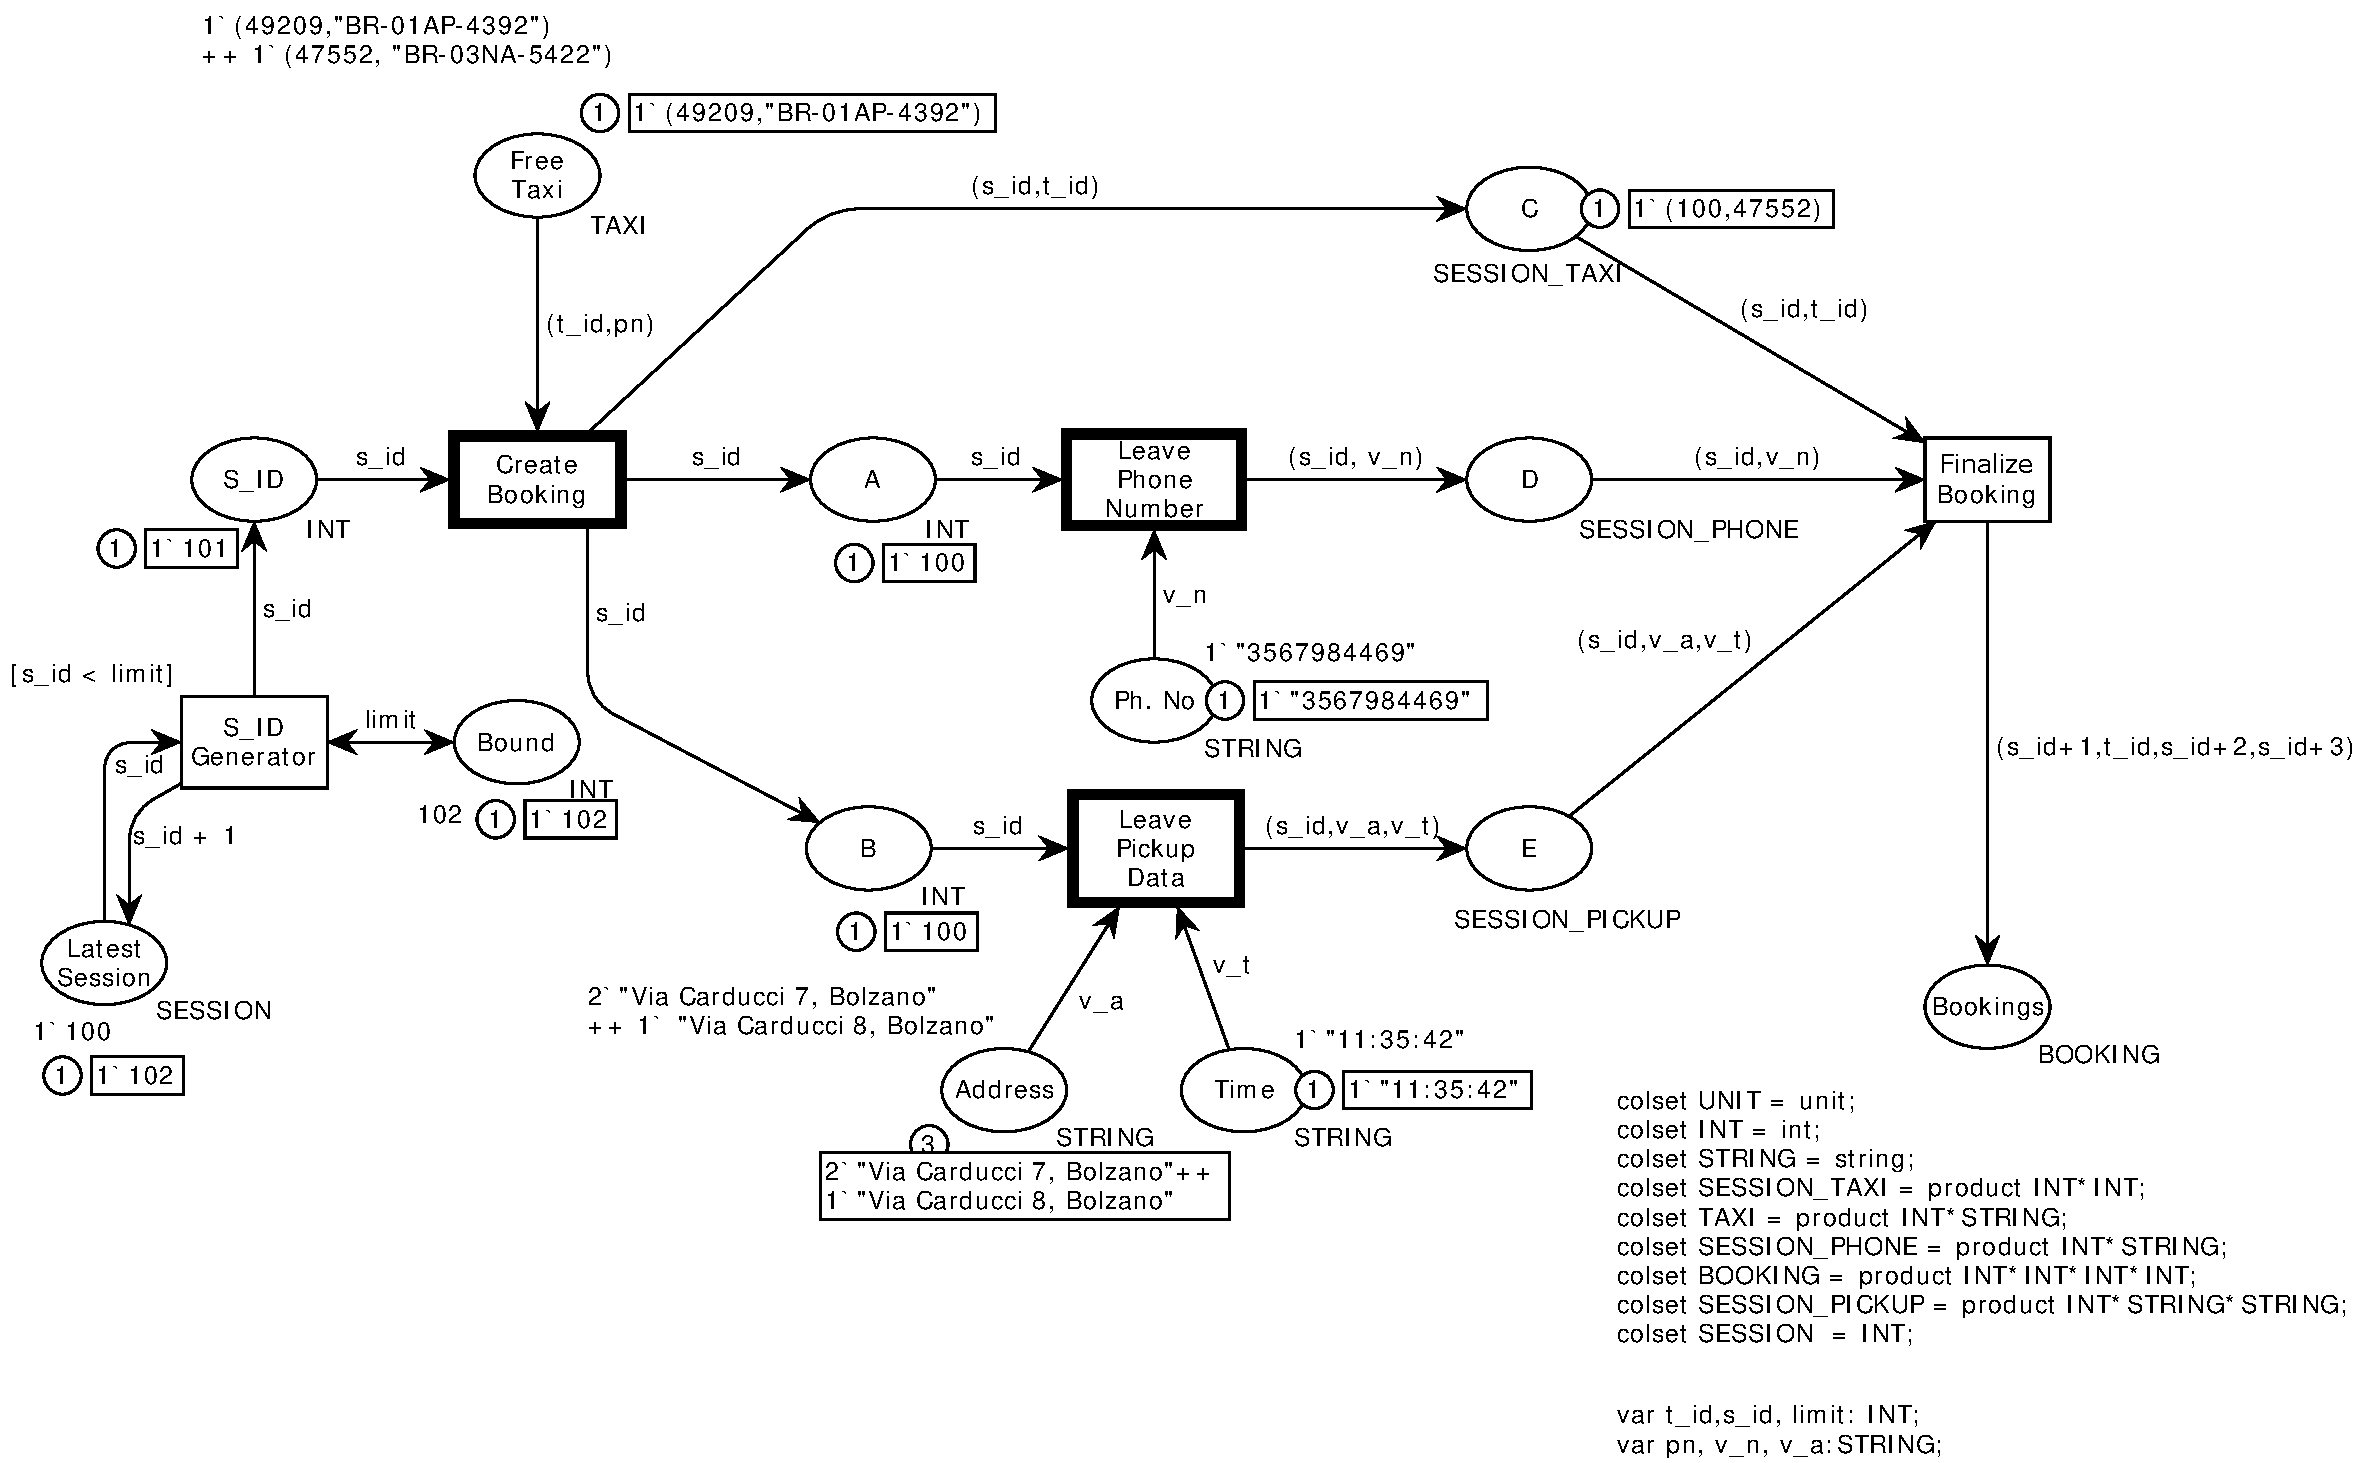
\includegraphics[scale = 0.35]{CPN_Taxi_Booking_one_step.pdf}
	\caption{A state of the CPN model for taxi booking}
	\label{fig:CPN_Taxi_Booking_one_step}
\end{figure}

\subparagraph*{\textnormal{In Figure \ref{fig:CPN_Taxi_Booking_one_step}, there are 3 transitions which are enabled, namely, $\mathit{Create\ Booking}$, $\mathit{Leave\ Phone\ Number}$ and $\mathit{Leave\ Pickup\ Data}$. This is the synchronization property of CPNs where there are multiple transitions enabled and each such transition may fire. The simulation(execution of transitions) is halted when there are no more enabled transitions.}}

\subparagraph*{\textnormal{Now with the explanation of how we can determine enabling and occurrence of steps, let us visit the definition of enabling and occurrence of a binding element in a coloured Petri net.}}
\begin{defs}
	\label{defs:enabling_binding_cpn}
	A binding element $\mathit{(t,b) \in BE}$ is \textbf{enabled} in a marking $\mathit{M}$ if and only
	if the following two properties are satisfied:
	\begin{enumerate}
		\item $\mathit{G(t)\langle b \rangle}$.
		\item $\mathit{\forall p \in P : E(p,t)\langle b \rangle \ll= M(p)}$.
		\item When $\mathit{(t,b)}$ is enabled in $\mathit{M}$, it may \textbf{occur}, leading to the marking $\mathit{M}$ defined by:
		\begin{equation*}
			\forall p \in P : M'(p) = \left(M(p) -\!- E(p,t)\langle b \rangle \right) +\!\!+ E(t, p)\langle b \rangle.
		\end{equation*}
	\end{enumerate}
\end{defs}

\subparagraph*{\textnormal{We have already covered enabling and occurrence of bindings. Now let us consider the enabling and occurrence of steps. In a step $\mathit{Y}$, each binding element (included in the step) should satisfy the guard of the transition $t$. Also, each place $\mathit{p}$ must have the marking $\mathit{M(p)}$ greater than or equal to the sum of the tokens that are removed from $\mathit{p}$.
		\begin{equation*}
		^{++}_{MS} \sum\limits_{(t,b) \in Y} E(p,t)\langle b \rangle \ll= M(p)
		\end{equation*}
		where MS to the lower left of the summation symbol specifies that
		we are adding a multiset of multisets. Each term $E(p, t)\langle b \rangle$ occurs as many times in the sum as $(t,b)$ occurs in $Y$.}}

\subparagraph*{\textnormal{The new marking $\mathit{M'}$ reached when an enabled step $\mathit{Y}$ occurs in a
		marking $\mathit{M}$ is given by:
		\begin{equation*}
			M'(p) = \left(M(p) -\!- ^{++}_{MS} \sum\limits_{(t,b) \in Y} E(p,t)\langle b \rangle \right)\ +\!\!+\ ^{++}_{MS}\sum\limits_{(t,b) \in Y} E(t,p)\langle b \rangle \forall p \in P
\end{equation*}}}

\subparagraph*{\textnormal{The state of the model after firing the transition $\mathit{Create\ Booking}$ with the binding $\mathit{b_{CB}}$ is shown in Figure \ref{fig:CPN_Taxi_Booking_one_step}. In a summarized way let us call the markings at this state of the system as $\mathit{M_{1}}$.
\begin{equation*}
M_{1}(p) = \begin{cases}
\textnormal{${1}^{\backprime}$101} & \textit{if p = S\_ID}\\
\textnormal{${1}^{\backprime}$(49209,\bdsq{BR-01AP-4392})}  & \textit{if p = Free Taxi}\\
\textnormal{${2}^{\backprime}$\bdsq{Via Carducci 7, Bolzano}} +\!\!+ & \textit{if p = Address}\\ 
\textnormal{${1}^{\backprime}$\bdsq{Via Carducci 8, Bolzano}} & \\
\textnormal{${1}^{\backprime}$\bdsq{11:35:42}} & \textit{if p = Time}\\
\textnormal{${1}^{\backprime}$\bdsq{3567984469}} & \textit{if p = Ph. No}\\
\textnormal{${1}^{\backprime}$100} & \textit{if p $\in$ \textnormal{\{}A, B\textnormal{\}}}\\
\textnormal{${1}^{\backprime}$(100,47552)} & \textit{if p = C}\\
\textnormal{${1}^{\backprime}$102} & \textit{if p = Latest Session}\\
\textnormal{${1}^{\backprime}$102} & \textit{if p = Bound}\\
\emptyset_{MS} & \textit{otherwise}
\end{cases}
\end{equation*}
The enabling and occurrence of a step can be defined as below:}}
\begin{defs}
	\label{defs:enabling_steps_cpn}
	A step $\mathit{Y \in BE_{MS}}$ is \textbf{enabled} in a marking $\mathit{M}$ if and only if the following
	two properties are satisfied:
	\begin{enumerate}
		\item $\mathit{\forall (t,b) \in Y : G(t)\langle b \rangle}$.
		\item $\mathit{\forall p \in P :\ ^{++}_{MS} \sum\limits_{(t,b) \in Y} E(p,t)\langle b \rangle \ll= M(p)}$
		\item When $\mathit{Y}$ is enabled in $\mathit{M}$, it may \textbf{occur}, leading to the marking $\mathit{M'}$ defined by:
		\begin{equation*}
			\forall p \in P : M'(p) = \left(M(p) -\!- ^{++}_{MS} \sum\limits_{(t,b) \in Y} E(p,t)\langle b \rangle \right)\ +\!\!+\ ^{++}_{MS}\sum\limits_{(t,b) \in Y} E(t,p)\langle b \rangle
		\end{equation*}
	\end{enumerate}
\end{defs}

\subparagraph*{\textnormal{Now we represent that the marking $\mathit{M_{2}}$ is directly reachable from $\mathit{M_{1}}$ by the step $\mathit{Y}$ by :
		\begin{center}
			$\mathit{M_{1} \xrightarrow{Y} M_{2}}$ or simply by $\mathit{M_{1} \xrightarrow{} M_{2}}$
		\end{center}
}}
\begin{defs}
	\label{defs:finite_occurrence_seq}
	A \textbf{finite occurrence sequence of length} $\mathit{n \geq 0}$ is an alternating sequence
	of markings and steps, written as
	\begin{equation*}
		M_{1} \xrightarrow{Y_{1}} M_{2} \xrightarrow{Y_{2}} M_{3} \ldots M_{n} \xrightarrow{Y_{n}} M_{n+1}
	\end{equation*}
	such that $\mathit{M_{i} \xrightarrow{Y_{i}} M_{i+1}}$ for all $\mathit{1 \leq i \leq n}$. All markings in the sequence are said to
	be \textbf{reachable} from $\mathit{M_{1}}$. This implies that an arbitrary marking $\mathit{M}$ is reachable from
	itself by the trivial occurrence sequence of length 0.\\
	Analogously, an \textbf{infinite occurrence sequence} is a sequence of markings and
	steps
	\begin{equation*}
		M_{1} \xrightarrow{Y_{1}} M_{2} \xrightarrow{Y_{2}} M_{3} \xrightarrow{Y_{3}} \ldots
	\end{equation*}
	such that $\mathit{M_{i} \xrightarrow{Y_{i}} M_{i+1}, \forall i \geq 1}$. The set of markings reachable from a marking $\mathit{M}$ is denoted $\mathit{\mathscr R(M)}$. The set of \textbf{reachable markings} is $\mathit{\mathscr R(M_{0})}$, i.e., the set of markings reachable from the initial marking $\mathit{M_{0}}$.
\end{defs}

\paragraph*{State Spaces}
\subparagraph*{\textnormal{The \textit{state space} of a CPN model is a directed graph $\mathit{SS}$, comprising a set of nodes $\mathit{N_{SS}}$ which corresponds to set of reachable markings $\mathit{\mathscr R(M_{0})}$ and a set of directed arcs represented by $\mathit{A_{SS}}$. An arc $\mathit{a \in A_{SS}}$ connects two nodes $\mathit{M}$ and $\mathit{M^{'}}$ and has a label of binding element $\mathit{(t,b)}$ on it iff $\mathit{(t,b)}$ is enabled in marking $\mathit{M}$ and occurrence of $\mathit{(t,b)}$ leads to the marking $\mathit{M^{'}}$, i.e., $\mathit{M \xrightarrow{(t,b)} M^{'}}$. The state space is finite if the set of reachable markings is finite and the set of enabled bindings in each reachable marking is also finite. The formal definition of the state space for a CPN model is:}}
\begin{defs}
	\label{defs:state_space}
	The \textbf{state space} of a Coloured Petri Net is a directed graph $\mathit{SS =
	(N_{SS},A_{SS})}$ with arc labels from BE, $\mathit{M_{0}}$ is the initial marking and M being an intermediate marking, where:
	\begin{enumerate}
		\item $\mathit{N_{SS} = \mathscr R(M_{0})}$ is the set of \textbf{nodes}.
		\item $\mathit{A_{SS} = \{ (M,(t,b),M^{'}) \in N_{Ss} \times BE \times N_{SS}\ | M \xrightarrow{(t,b)} M^{'} \}} $ is the set of \textbf{arcs}.
	\end{enumerate}
	$SS$ is finite if and only if $\mathit{N_{SS}}$ and $\mathit{A_{SS}}$ are finite.
\end{defs}

\subparagraph*{\textnormal{For the CPN model in Figure \ref{fig:CPN_Taxi_Booking}, there are more than 50 nodes and more than 100 arcs in the state space which makes it difficult to show all the states. For simplicity, we slightly change our model and our new model is shown in Figure \ref{fig:CPN_Taxi_Booking_simple}. In this model, we removed the transition \textit{S\_ID Generator} and fixed the assume that only a single session identifier is generated. Also, for simplicity, some tokens are removed from the place \bsq{Address}. While drawing the state space, we label the nodes with the marking of the model and arcs with the fired transition and the corresponding binding element. The state space of this CPN model is shown in Figure \ref{fig:CPN_State_Space}.}}

\subparagraph*{\textnormal{In Figure \ref{fig:CPN_State_Space}, in case of node 1, markings of all places are written, however, due to the large size of the state space, the marking of each node is not shown. Hence we only write the marking of the places which do not have empty marking.}}

\begin{comment}
For example, at node 2, the marking of the place \bsq{S\_ID} is $\emptyset_{MS}$, hence we omit its marking at node 2. Similarly at node 2, the marking of the places \bsq{D} and \bsq{E} is $\emptyset_{MS}$, hence their markings are also omitted.
\end{comment}

\subparagraph*{\textnormal{Node 1 represents the initial state of the model. From node 1, taking any one of the free taxis (there are two taxis available), one can go to either node 2 or to node 3. From node 2, the customer has the option to provide pickup data first and then the phone number or vice versa. Depending on the choice we reach node 4 or node 5. If we provided phone number at the first place then we need to provide the pick up data, else we need to provide the phone number. This leads us to node 8. From node 8, we could add/finalize the booking which leads us to node 10. Similarly, one could go from node 3 and expand it. At node 10, there are no more transitions enabled hence there are no more arcs emerging from them. In this case, $\mathit{N_{SS}}$ (set of nodes of state space) and $\mathit{A_{SS}}$ (set of arcs of state space) are finite, hence the state space is also finite.}}

\begin{figure}[!htbp]
	\centering
	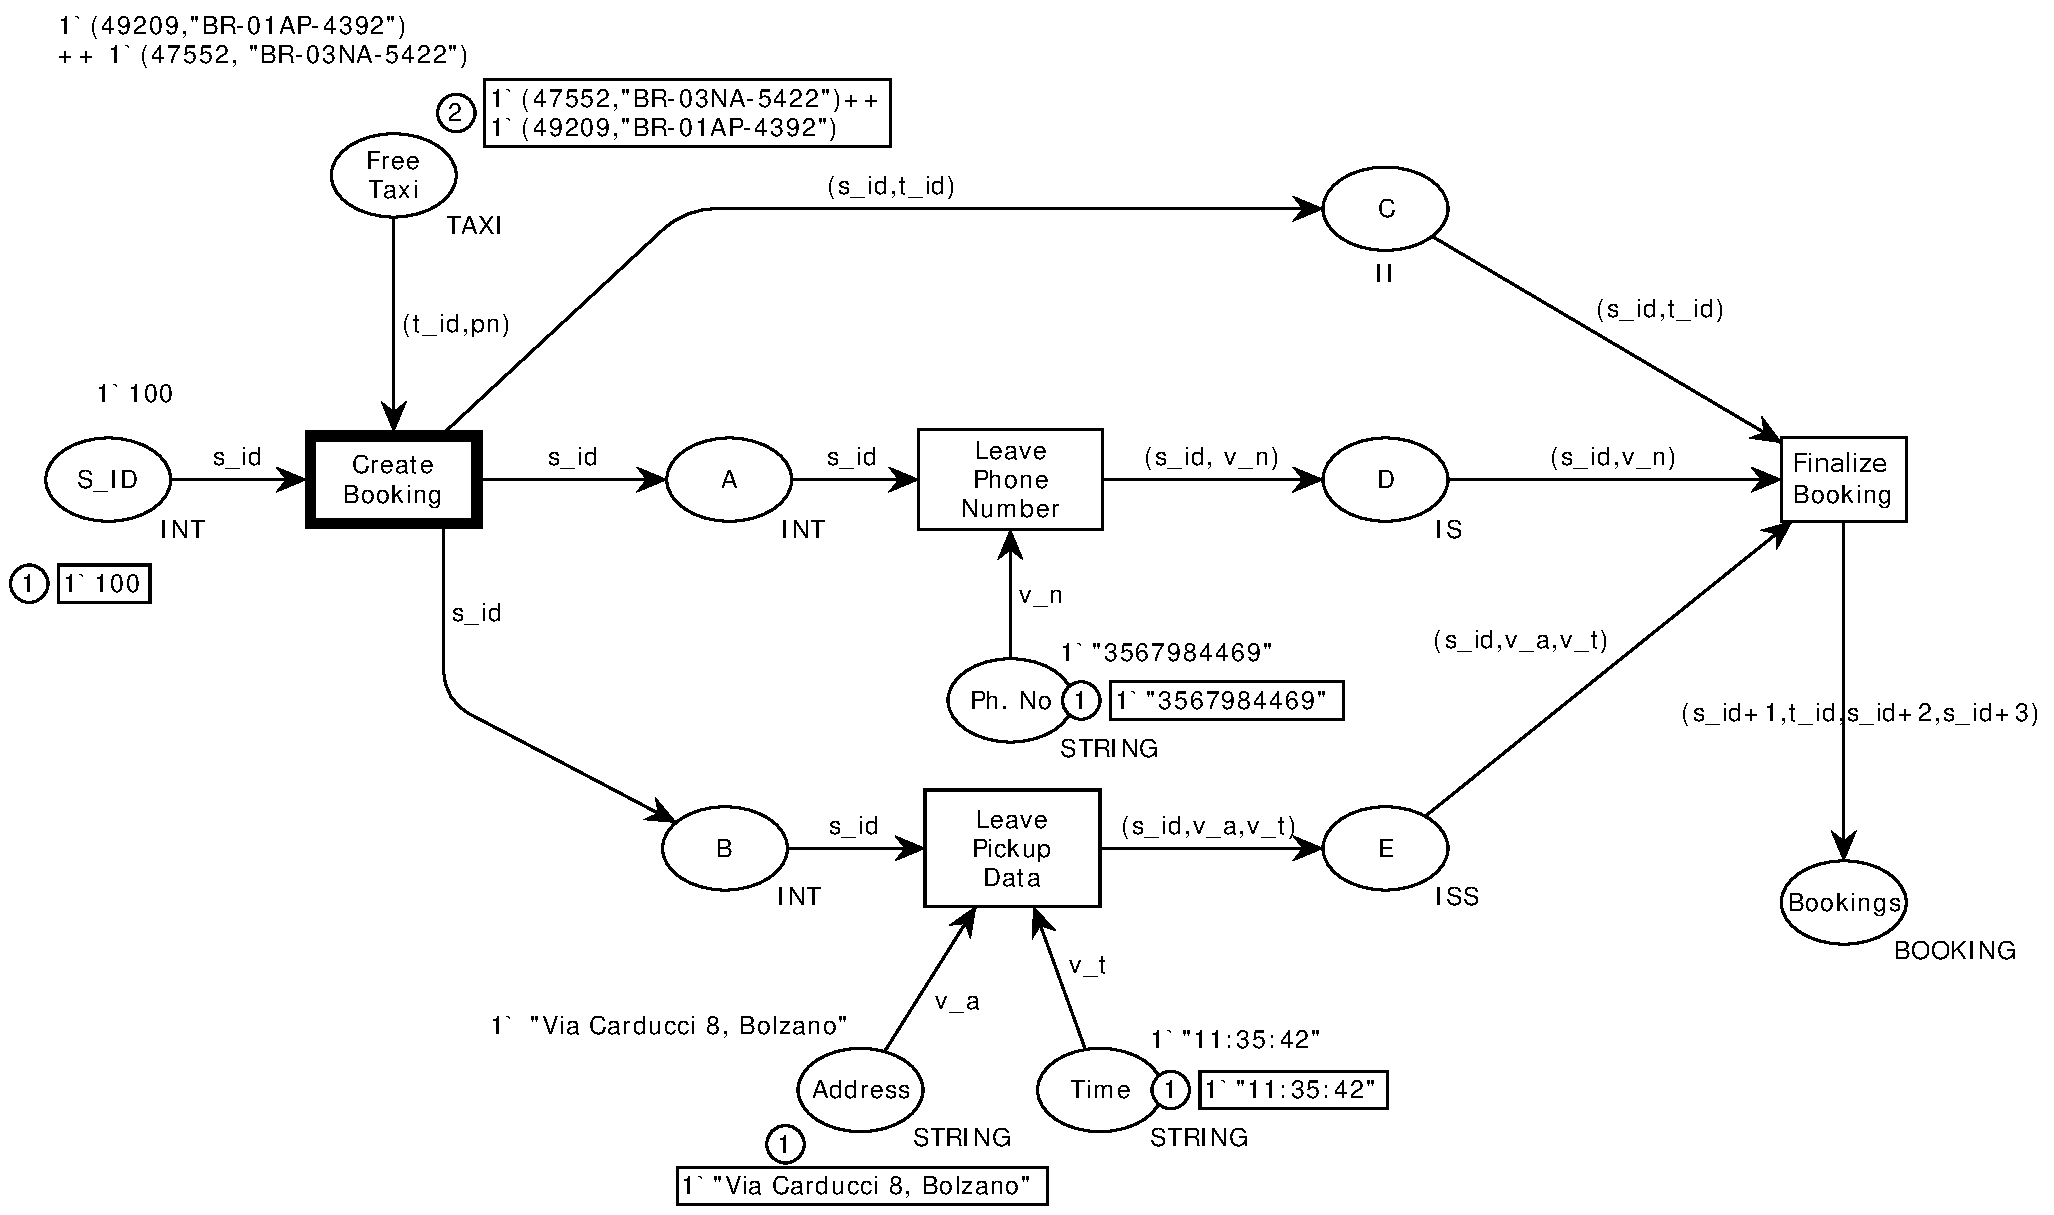
\includegraphics[scale = 0.4]{CPN_Taxi_Booking_simple.pdf}
	\caption{Revised CPN model showing a state for taxi booking example}
	\label{fig:CPN_Taxi_Booking_simple}
\end{figure}

\begin{figure}
	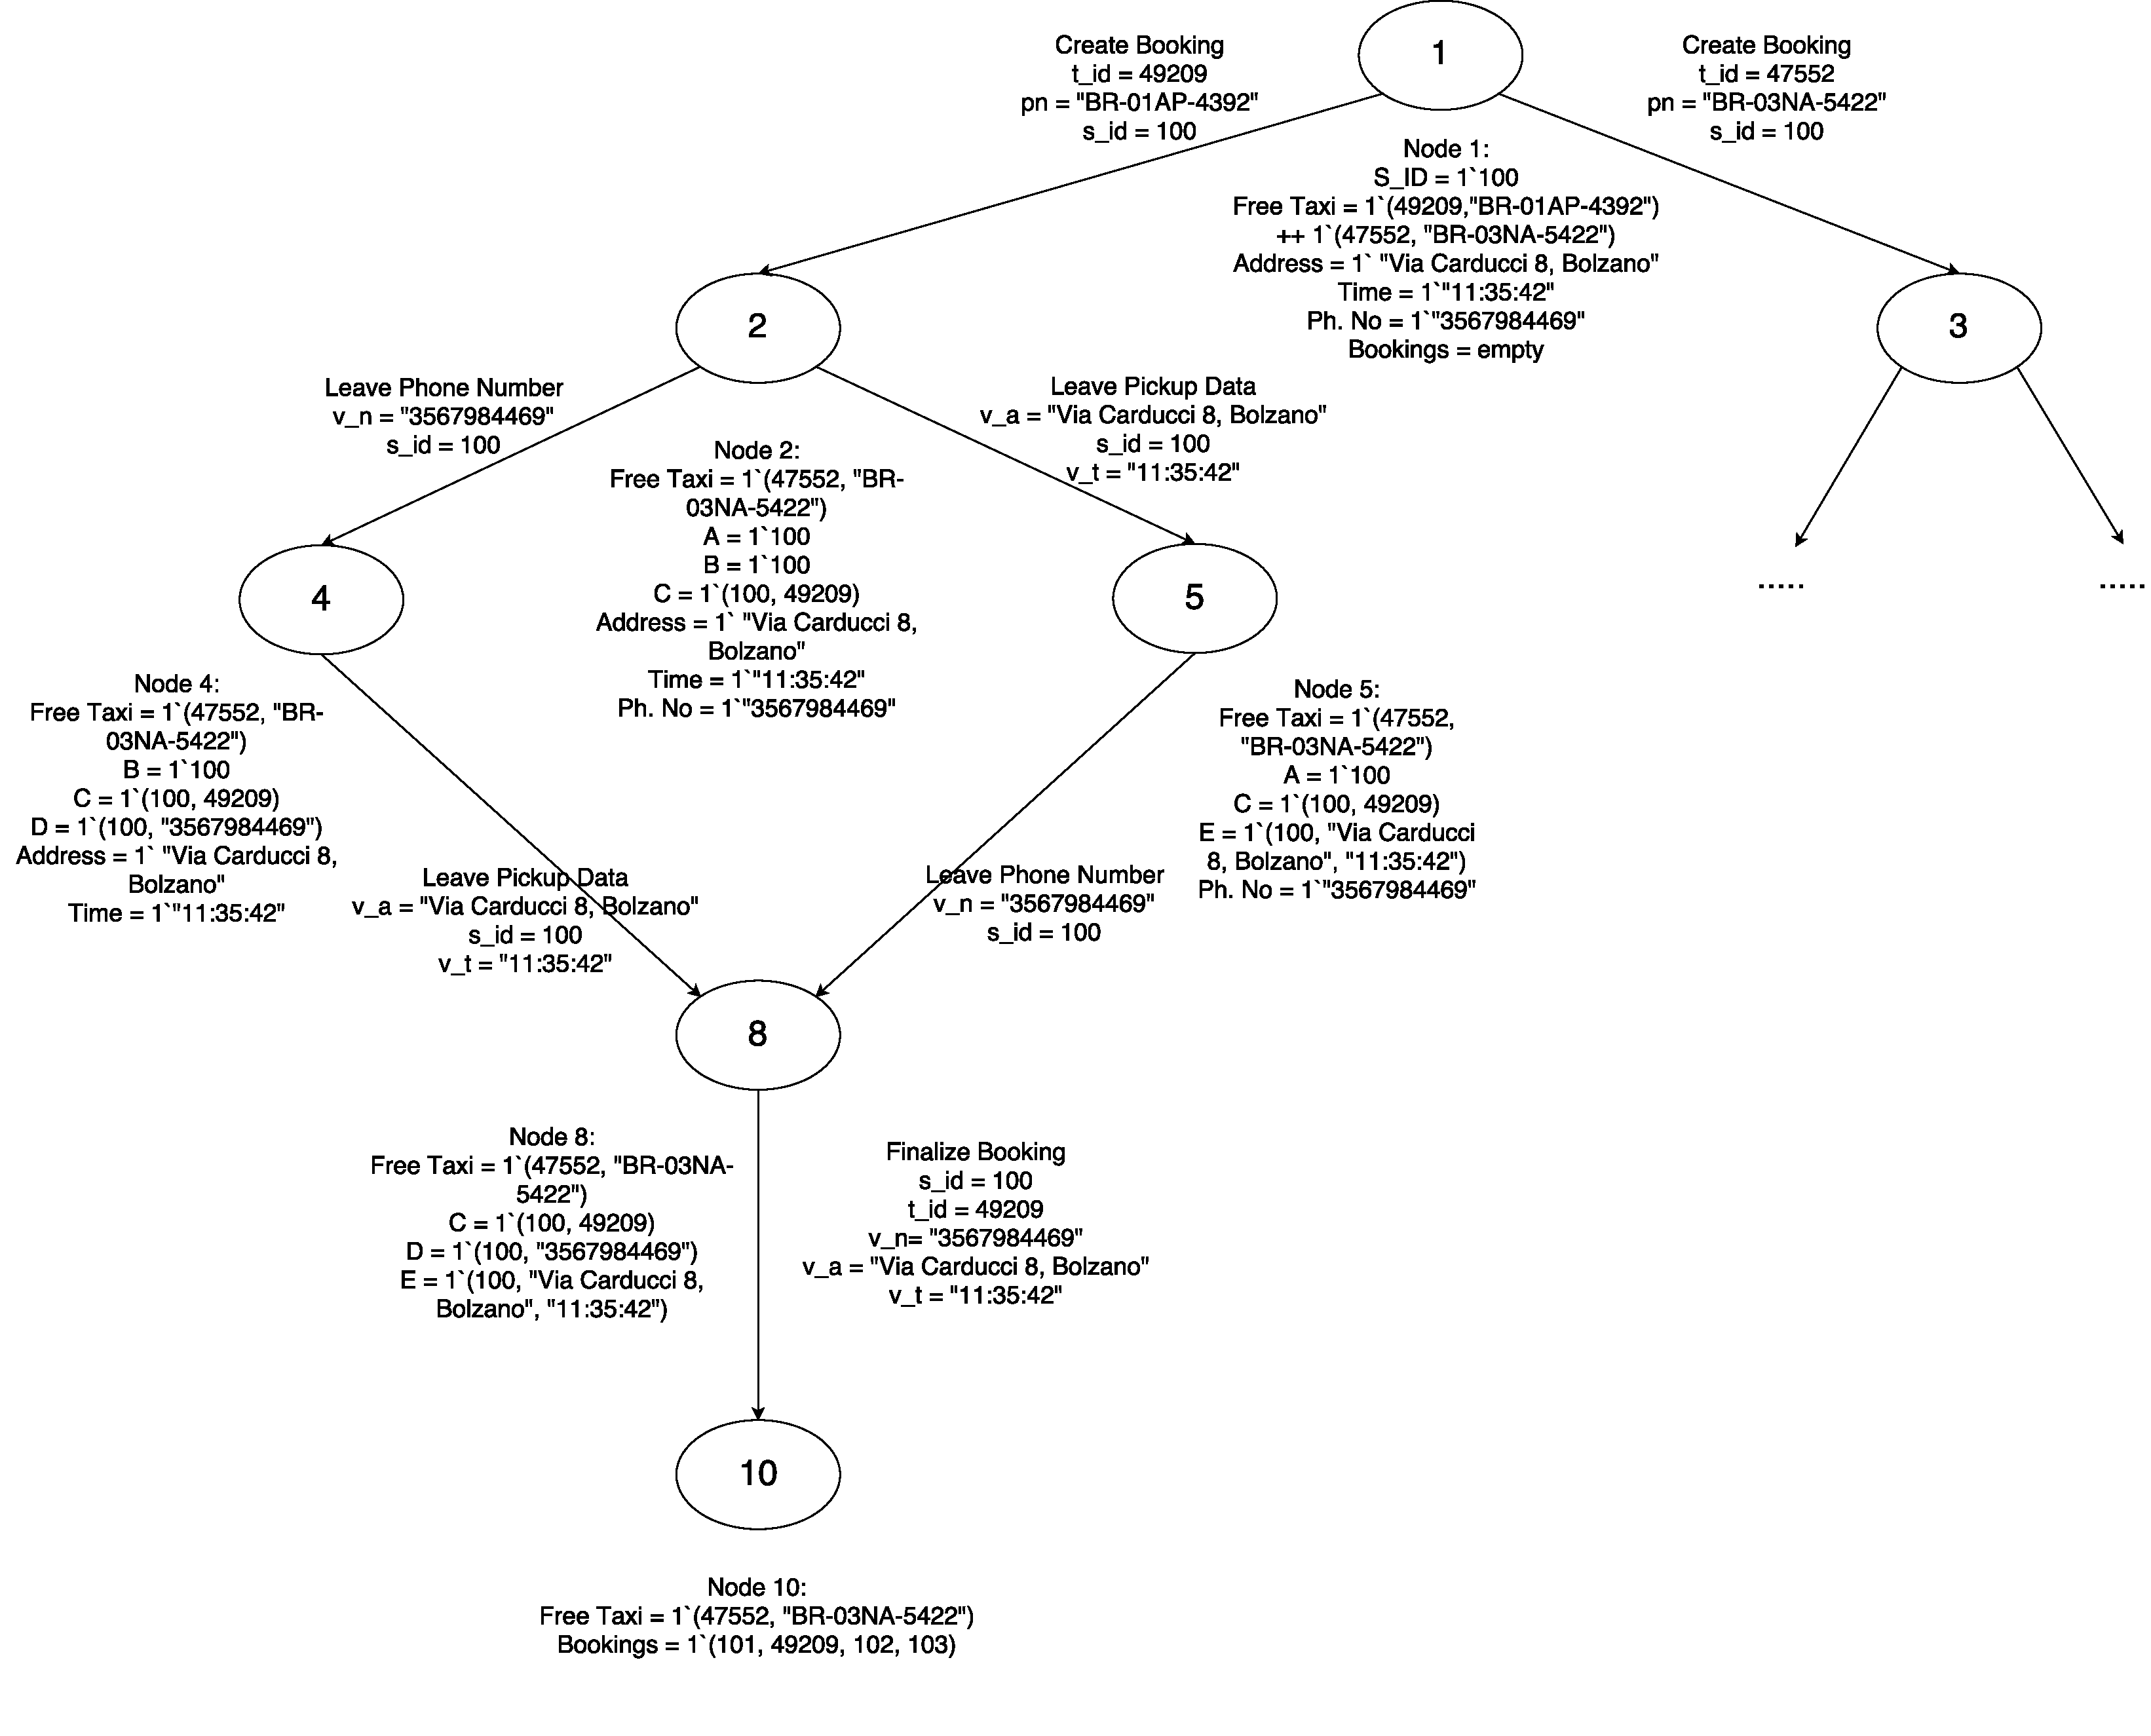
\includegraphics[scale = 0.21]{CPN_Taxi_Booking_State_Space.pdf}
	\caption{State Space for CPN model in Figure \ref{fig:CPN_Taxi_Booking_simple}}
	\label{fig:CPN_State_Space}
\end{figure}

%\graphicspath{{./images/DBN/}}
\chapter{Extending CPN with Relational Data}
\label{ch:EXT_CPN_RDB}
\paragraph*{\textnormal{This chapter presents an extension of CPN with relational data. An attempt to integrate master data with processes, made by Montali and Rivkin in \cite{DBLP:journals/corr/DBNets}, is presented in this chapter. In this chapter, we will see how coloured petri nets can be extended in order to incorporate relational data. We first give an idea about different layers of DB-nets and how they are interconnected. Later, we will walk through the taxi booking example and modify it to adjust to a DB-net model. Finally, we model the developed DB-net model into CPN Tools. The example for the taxi booking model presented in this chapter is taken from \cite{DBLP:journals/corr/DBNets}.}}

\section{DB-Nets}
\paragraph*{\textnormal{In this section we will build up on the taxi booking example provided in the previous chapter. In this example, the process experts\footnote{process experts are people who are experts on modelling processes.} focus on how the process of booking a taxi is carried out. They may use the petri net model (informally presented in Figure \ref{fig:DBN_PN_Informal}) in order to represent the business process and its requirements, whereas on the other hand the master data experts would take care of requirements about the relevant data of the domain. Then, one can structure the data into classes, provide relationship, constraint etc in order to draft a database schema (informally represented in Figure \ref{fig:DBN_DataModel_Informal}).}}
\begin{figure}[!htbp]
	\centering
	\begin{subfigure}{0.5\textwidth}
		\centering
		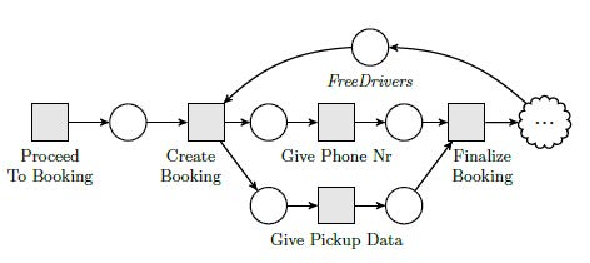
\includegraphics[width=1.0\linewidth]{DBN_PN_Informal.pdf}
		\caption{Process Model}
		\label{fig:DBN_PN_Informal}
	\end{subfigure}%
	\begin{subfigure}{0.5\textwidth}
		\centering
		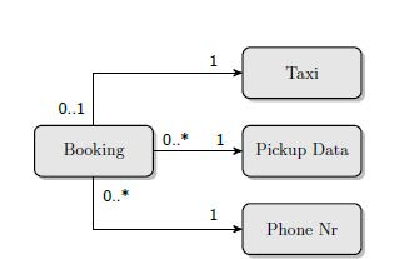
\includegraphics[width=0.7\linewidth]{DBN_DataModel_Informal.pdf}
		\caption{Data Model}
		\label{fig:DBN_DataModel_Informal}
	\end{subfigure}
	\caption{Figure \ref{fig:DBN_PN_Informal} captures the process part informally whereas figure \ref{fig:DBN_DataModel_Informal} captures the data model informally for the taxi booking example.}
	\label{fig:DBN_informal_model}
\end{figure}

\subparagraph*{\textnormal{The problem of integration lies in the example, that in the process flow, while encountering the \textit{Create Booking} transition the process expert would think to create a booking (i.e. instantiate the booking class), whereas from the schema, a booking can only exist in the database only if the corresponding taxi, phone number and the pickup address is provided. With this prospect, during execution one could keep track of free taxi, pickup data and phone number using local variables, and when \textit{Finalize Booking} is called, the corresponding booking entry is created. In this regard, we introduce DB-Nets. In Figure \ref{fig:DBN_Framework}, the framework of the db-nets is presented.}}

\begin{figure}[!htbp]
	\centering
	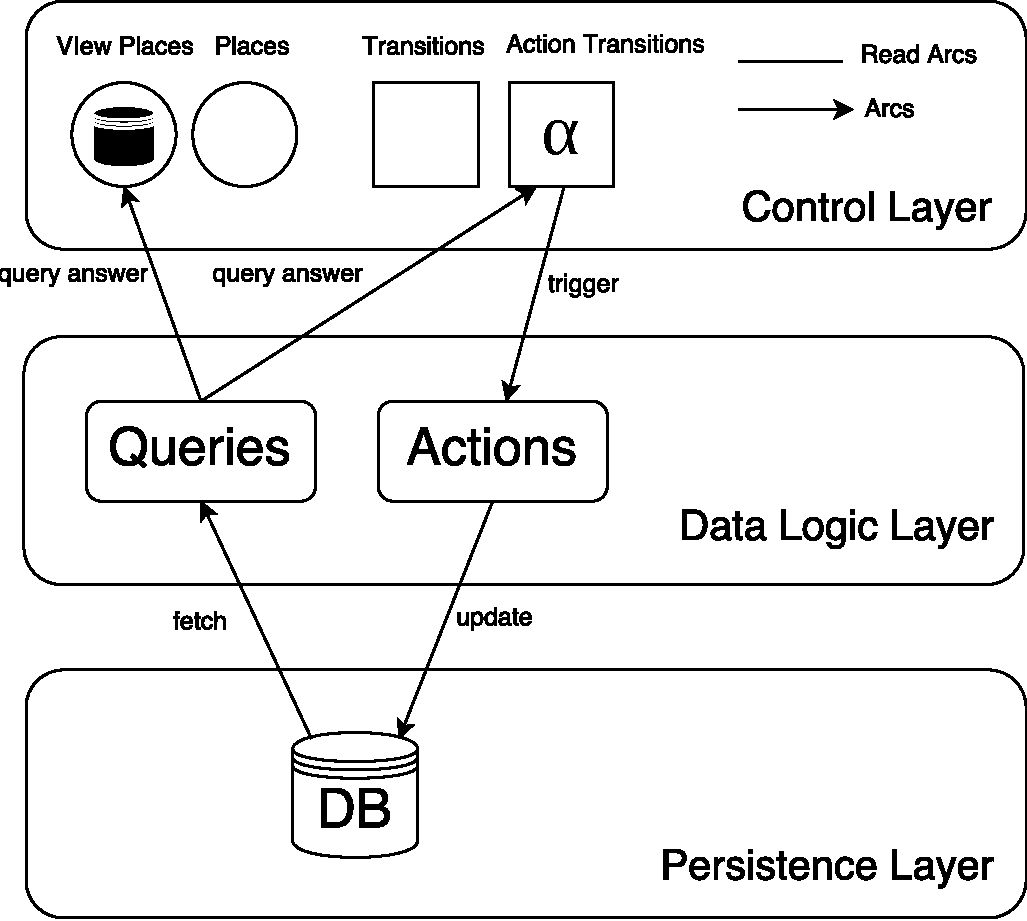
\includegraphics[scale = 0.35]{DBN_Framework.pdf}
	\caption{Framework of the DB-Net model}
	\label{fig:DBN_Framework}
\end{figure}

\subparagraph*{\textnormal{As per \cite{DBLP:journals/corr/DBNets}, the framework comprises of the three layers which are as follows:
		\begin{itemize}
			\item Persistence Layer - contains the full-fledged relational database with constraints. 
			\item Control Layer - process logic is represented with the help of a variant of CPN which supports:
			\begin{enumerate}
				\item typing of tokens, so
				as to account for local variables attached to execution threads.
				\item injection of possibly fresh data values via special so-called $\mathit{\nu}$-variables (leveraging the $\mathit{\nu}$-PN
				model \cite{DBLP:journals/tcs/Rosa-VelardoF11}).
				\item accessing the content of the underlying data layer via special	\textbf{\textit{view-places}}.
				\item updating the underlying data layer by attaching a database update logic to its transitions.
			\end{enumerate} 
			\item Data Logic Layer - used to connect the persistence and the control layer.
		\end{itemize}
}}
\subparagraph*{\textnormal{In figure \ref{fig:DBN_Framework}, the control layer contains a special place called view place, special transitions called action transitions and special arcs called read arcs. The control layer makes use of these special elements to interact with data logic layer in a bidirectional way.}}

\begin{comment}
If we don't intend to consume tokens from a place, then we connect the place with the read arc. The read arc just reads the token value and doesn't remove token from the connected place. The role of rollback arc is to undo the effect of a transition. We would discuss more about this later in the chapter.
\end{comment}

\subparagraph*{\textnormal{The db-net model of the taxi booking example is shown in Figure \ref{fig:DBN_Taxi_Example}. In this example, we assume that from some workflow  \textit{Proceed To Booking} transition is called. Similarly, after the booking is added there may be another workflow. In this example, we are only concerned about the workflow of booking a taxi. Let us see how the three layers (mentioned in the in figure \ref{fig:DBN_Framework}) can be interpreted in the given example (figure \ref{fig:DBN_Taxi_Example}).}}

\begin{figure}[!htbp]
	\centering
	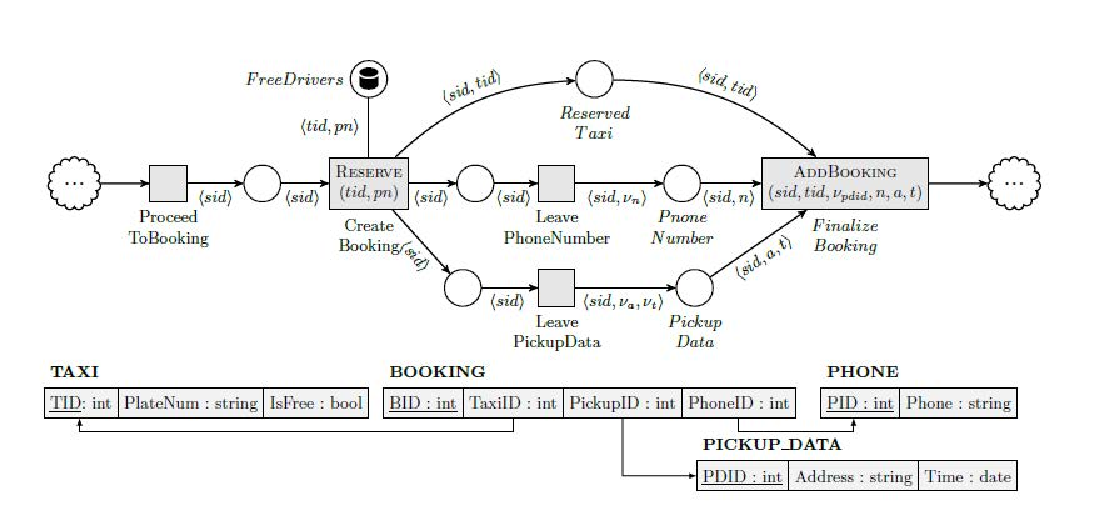
\includegraphics[scale = 0.8]{DBN_Taxi_Example.pdf}
	\caption{A db-net representing the taxi booking process}
	\label{fig:DBN_Taxi_Example}
\end{figure}

\subsubsection{Persistence Layer}
\begin{comment}
\paragraph*{\textnormal{Persistence layer consists of a full-fledged relational databases including constraints. For example, in figure \ref{fig:DBN_Taxi_Example}, the persistence layer consists of the database which contains table \bsq{\textbf{TAXI}}, \bsq{\textbf{BOOKING}}, \bsq{\textbf{PHONE}} and \bsq{\textbf{PICKUP\_DATA}}. The \bsq{TAXI} table consists of 3 columns \bsq{TID} containing integers, \bsq{PlateNum} containing strings and \bsq{IsFree} which contains the boolean value. If a taxi is available then its corresponding record in the \bsq{TAXI} table will have the column $IsFree = \textit{True}$. \bsq{PHONE} table consists of columns \bsq{PID} containing integers and \bsq{Phone} containing the phone numbers as strings. \bsq{PID} is the phone id for a particular phone number. \bsq{PICKUP\_DATA} table contains the pickup data for the customer. The columns in this table are \bsq{PDID} which contains integer, \bsq{Address} containing pickup address as string and \bsq{Time} of type date. \bsq{PDID} is the pickup id for a particular customer's pickup details (address and time). The table \bsq{BOOKING} contains the column \bsq{BID} as integer, \bsq{TaxiID} as integer, \bsq{PickupID} as integer and \bsq{PhoneID} as integer. For a particular record in the \bsq{BOOKING} table, \bsq{BID} denotes the corresponding booking id.}}

\subparagraph*{\textnormal{Along with the table structure, we have also introduced the constraints over it. For example, in the taxi table, a particular \bsq{TAXI} can be uniquely determined from \bsq{TID}. Hence, \bsq{TID} is the primary key (underlined in the figure \ref{fig:DBN_Taxi_Example}). Similarly, each phone number in the \bsq{PHONE} table can be determined by \bsq{PID} and in the table \bsq{PICKUP\_DATA} the pickup details can be determined by \bsq{PDID}. So, these two columns are marked as primary keys. In the \bsq{BOOKING} table, each booking can be determined by \bsq{BID}. \bsq{TaxiID}, \bsq{PickupID} and \bsq{PhoneID} are the foreign keys to the columns \bsq{TID}(in the \bsq{TAXI} table), \bsq{PDID}(in the \bsq{PICKUP\_DATA} table) and \bsq{PID}(in the \bsq{PHONE} table) respectively. This constraints will allow a booking to be added only if it has its corresponding \bsq{TaxiID}, \bsq{PickupID} and \bsq{PhoneID} in the \bsq{TAXI}, \bsq{PICKUP\_DATA} and \bsq{PHONE} table respectively.}}
\end{comment}

\subparagraph*{\textnormal{The persistence layer stores the relevant data for the domain of interest. We consider the relational databases along with its constraints. Using FOL we can express keys, functional dependencies and constraints over the database \cite{BagheriHariri}. For example, in Figure \ref{fig:DBN_Taxi_Example}, different tables are shown along with their functional dependencies and keys. A slight modification in persistence layer is presented in \cite{DBLP:journals/corr/DBNets}.}}

\subparagraph*{\textnormal{As mentioned in the preliminaries (section \ref{sec:preliminaries_relational_db_schema}), we consider the notion of relational schema, sort function and database schema for our need. }}

\begin{comment}
\subparagraph*{\textnormal{We will start with the definition of data type and adopt database schema and relational schema accordingly.}}
\subparagraph*{\textnormal{\todo{here these notions come out of the blue}Inspired from \cite{DBLP:books/aw/found_DB}, we assume \textit{domain} as a countably infinite set $\mathit{\Delta}$, \textit{attributes} as a finite set \textit{\mathit{U}}, and a mapping function $\mathit{dom:U\rightarrow\Delta$ and $dom(A)}$ is called domain of $\mathit{A}$, where $\mathit{A \in U}$.}}

\begin{defs}
\label{defs:dbn_sort_function}
\todo{for all the definitions, please, read carefully page 31 of the cited book. also, try to add more details to your definitions. for example, what does a finitary powerset mean?}
A function \textit{sort} is defined as $sort:R^{n}\rightarrow{\mathcal{P}^{fin}}(U)$, where ${\mathcal{P}^{fin}}$ is the finitary powerset\footnote{the set of finite subsets} of attributes, $R^{n}$ is the set of relation schema and $U$ is the finite set of attributes.
\end{defs}

\subparagraph*{\textnormal{The sort of a relation schema \textit{\mathit{R}} is simply written as $\mathit{sort(R)}$ and the arity is written as $\mathit{arity(R) = |sort(R)|}$. A relational schema ($\mathit{R}$) and set of attributes($\mathit{U}$) together make up the structure of the table. $\mathit{R[U]}$ is used to represent $\mathit{sort(R) = U}$, and $\mathit{R[n]}$ to represent $\mathit{arity(R) = n}$.}}

\begin{defs}
\label{defs:dbn_database_schema}
For a given domain $\Delta$, a \textbf{database schema}\todo{you haven't defined a type function for the database schema} is a non empty finite set $\mathcal{R}$ of relational schemas, written as:
\begin{equation*}
\mathcal{R} = \{R_{1}[U_{1}],\ldots,R_{n}[U_{n}]\}
\end{equation*}
where $R_{1},\ldots,R_{n}$ are relational schemas and $U_{1},\ldots,U_{n}$ are attributes
\end{defs}

\subparagraph*{\textnormal{For example, let \textbf{\textit{taxi\_booking}} be our database schema, shown in Figure \ref{fig:DBN_CPNTools_Taxi_Example}, which is defined by:
\begin{equation*}
\begin{aligned}
\textbf{\textit{taxi\_booking}} =& \{TAXI,\ BOOKING,\ PHONE,\ PICKUP\_DATA\}
\end{aligned}
\end{equation*}
where relational schemas TAXI and PHONE\footnote{One could also write sorts for other relation schemas in the $\textbf{taxi\_booking}$ schema} have the following sorts:
\begin{equation*}
\begin{aligned}
sort(TAXI) = & \{TID,\ PlateNum,\ IsFree\}\\
sort(PHONE)= & \{PID,\ Phone\}
\end{aligned}
\end{equation*}
}}

\subparagraph*{\textnormal{We assume that a \textit{data type} is an infinite set and is defined in a set theoretic manner. For example, \textit{int}, \textit{strings} etc. are \textit{data types}. We define a finite set $\mathit{\Gamma}$ as the set of all data types.}}

\begin{defs}
	\label{defs:dbn_type_function_database}
	A function $\mathit{type_{d}:U \rightarrow \Gamma}$, where $\mathit{U}$ is the set of attributes and $\mathit{\Gamma}$ is the set of data types.
\end{defs}

\subparagraph*{\textnormal{Now we define a typed relational schema as:}}

\begin{defs}
	\label{defs:dbn_typed_relational_schema}
	Given a relation schema $\mathit{R}$ and $\mathit{type_{d}}$ function, a typed relation schema $\mathit{R_{\Delta}}$ is a pair $\mathit{\langle R, type_{d}\rangle}$. 
\end{defs}

\subparagraph*{\textnormal{We extend the notion of the function $\mathit{sort}$, and we define a function $\mathit{sort_{d}}$, such as: }}

\begin{defs}
	\label{defs:dbn_typed_sort_function}
	A function $\mathit{sort_{d}}$ is defined as $\mathit{sort_{d}:R_{\Delta}^{n}\rightarrow{\mathcal{P}^{fin}}(U)}$, where $\mathit{{\mathcal{P}^{fin}}}$ is the finitary powerset\footnote{the set of finite subsets} of attributes, $\mathit{R_{\Delta}^{n}}$ is the set of typed relation schema and $\mathit{U}$ is the finite set of attributes.
\end{defs}

\subparagraph*{\textnormal{The typed sort of a relation schema $\mathit{R_{\Delta}}$ is simply written as $\mathit{sort(R_{\Delta})}$ and the arity is written as $\mathit{arity(R_{\Delta}) = |sort(R_{\Delta})|}$. A typed relational schema ($\mathit{R_{\Delta}}$) and set of attributes($\mathit{U}$) together make up the structure of the table. $\mathit{R_{\Delta}[U]}$ is used to represent $\mathit{sort(R_{\Delta}) = U}$.}}

\begin{defs}
	\label{defs:dbn_typed_database_schema}
	For a given domain $\mathit{\Delta}$, the set of data types $\mathit{\Gamma}$, a \textbf{typed database schema} is a non empty finite set $\mathit{\mathcal{R}_{\Delta}}$ of relational schemas, written as:
	\begin{equation*}
	\mathcal{R}_{\Delta} = \{R_{\Delta_{1}}[U_{1}],\ldots,R_{\Delta_{n}}[U_{n}]\}
	\end{equation*}
	where $\mathit{R_{\Delta_{1}},\ldots,R_{\Delta_{n}}}$ are typed relational schemas and $\mathit{U_{1},\ldots,U_{n}}$ are attributes.
\end{defs}
\end{comment}

\subparagraph*{\textnormal{For example, let \textbf{\textit{taxi\_booking}} be our database schema($\mathcal{R}$), shown in Figure \ref{fig:DBN_Taxi_Example}, which is defined as:
		\begin{equation*}
		\begin{aligned}
		\textbf{\textit{taxi\_booking}} =& \{TAXI,\ BOOKING,\ PHONE,\ PICKUP\_DATA\}
		\end{aligned}
		\end{equation*}
		where relational schemas TAXI and PHONE\footnote{One could also write sorts for other relation schemas in the $\textbf{taxi\_booking}$ schema} have the following sorts and data types:
		\begin{equation*}
		\begin{aligned}
		sort(TAXI) = & \{TID,\ PlateNum,\ IsFree\}\\
		sort(PHONE)= & \{PID,\ Phone\}\\\\
		dom(TID) =\ & int\\
		dom(PlateNum)=\ & string
		\end{aligned}
		\end{equation*}
}}

\begin{defs}
	\label{defs:dbn_rfacts}
	Given a database schema $\mathit{\mathcal{R}}$, a typed relation schema $\mathit{R}$, \textbf{an $\mathit{\mathcal{R}}$ fact} is of the form $\mathit{R(o_{1},\ldots,o_{n})}$ such that $\mathit{o_{i}}$ is an element of a data type and $\mathit{arity(R) = n}$.
\end{defs}

\subparagraph*{\textnormal{Here we will consider a full-fledged typed database schema as our persistence layer.}}
\subsubsection{Data Logic Layer}
\paragraph*{\textnormal{Data Logic Layer is the bidirectional interface between the control layer and the persistence layer. With bidirectional interface, we mean that on one hand we could extract data from an instance of the typed database schema which can be used in the persistence layer where as on the other hand, we could update the instance of the typed database schema by adding and deleting multiple facts at once. If the new database instance obtained after the update is compliant with the persistence layer, the update is committed, otherwise it is rolled back.}}

\subparagraph*{\textnormal{In order to query the database, we use first order logic queries, whereas to update the database instance, we follow the literature on data-centric processes \cite{DBLP:conf/icdt/Vianu09,DBLP:conf/pods/CalvaneseGM13}, where \textit{actions} are used to update database.}}

\begin{defs}
	An \textbf{action} over a persistence layer is a tuple $\mathit{\langle \textbf{n},\vec{p},F^{+},F^{-}\rangle}$, where $\mathit{\textbf{n}}$ is the action name, $\mathit{\vec{p}}$ is a tuple of pairwise distinct typed variables, denoting the \textit{action parameters}, $\mathit{F^{+}}$ and $\mathit{F^{-}}$ respectively represents a finite set of $\mathit{\mathcal{R}_{\Delta}}$-facts over $\mathit{\vec{p}}$, to be added or deleted from the current database instance.
\end{defs}

\subparagraph*{\textnormal{In order to access different components of the action $\mathit{\alpha = \langle \textbf{n},\vec{p},F^{+},F^{-}\rangle}$, we use the dot wise notation: $\mathit{\alpha\cdot}$name = \textbf{n}, $\mathit{\alpha\cdot}$params = $\mathit{\vec{p}}$, $\mathit{\alpha\cdot}$add = $\mathit{F^{+}}$, $\mathit{\alpha\cdot}$del = $\mathit{F^{-}}$. The data logic layer provides a set of actions with which one could update the database instance along with querying the database. For example, on firing the \textit{Create Booking} transition which contains the \textit{RESERVE} action, the database is updated such that the selected taxi is no longer available. The \textit{RESERVE} action has two input parameters, namely \textit{tid} and \textit{pn} denoting taxi id and the plate number respectively. This could be modelled as:
\begin{equation*}
\begin{aligned}
&RESERVE\cdot\textnormal{params} = \langle tid,pn \rangle \\
&RESERVE\cdot\textnormal{del} = \{Taxi(tid,pn,TRUE)\} \\
&RESERVE\cdot\textnormal{add} = \{Taxi(tid,pn,FALSE)\} \\
\end{aligned}
\end{equation*}
The set of FOL queries attached with the actions helps us querying the database and obtain the result. For example, the transition $\mathit{Finalize\ Booking}$, adds a booking to the table \textit{BOOKING} with a unique booking id, which is obtained as an answer to the attached query.}}

\subparagraph*{\textnormal{The data logic layer captures the flow of information from the control layer and performs actions on it. Similarly, this layer is also responsible for receiving the answer to the query from the persistence layer and passing on to the control layer.}}

\subparagraph*{\textnormal{Note that in control layer, we modify the definition of colour-sets ($\mathit{\Sigma}$) and say that colour-sets ($\mathit{\Sigma}$) is the finite set of possibly infinite colour-set. This is intentionally done to make the colour-sets compatible with answers of the queries.}}

\subsubsection{Control Layer}
\paragraph*{\textnormal{ In Figure \ref{fig:DBN_Framework}, the control layer has few additional components, namely, \textit{View places}, \textit{Action Transitions} and \textit{Read arcs}. These components are also incorporated in Figure \ref{fig:DBN_Taxi_Example}. The place $\mathit{Free\ Drivers}$ is a \textit{view place} which shows the currently available taxis. Since the records of the free taxi are stored in the database, they are fetched as an answer on querying the database. The set of view places is represented by $\mathit{P_{v}}$.}}

\begin{defs}
	\label{defs:dbn_query_function}
	A function $\mathit{query_{v}}$ is defined as $\mathit{query_{v} : P_{v} \rightarrow Q}$ where $\mathit{Q}$ is the set of first order logic queries.
\end{defs}

\begin{defs}
	\label{defs:dbn_formal_view_place}
	The set of \textbf{view places} ($\mathit{P_{v}}$) is a set such that:
	\begin{enumerate}
		\item $\mathit{P_{v} \subseteq P}$.
		\item for each $\mathit{p_{v} \in P_{v}}$, $\mathit{query_{v}(p_{v}) = q}$ where $\mathit{q \in Q}$.
		\item the answer $\mathit{(a_{1},\ldots,a_{k})}$ to the query $\mathit{q}$ having free variables $\mathit{(x_{1},\ldots,x_{k})}$, for all $\mathit{p_{v} \in P_{v}}$, $\mathit{(a_{1},\ldots,a_{k}) \in C(p_{v})}$.
		\item Let $\mathit{Ans = \{A_{1}, \ldots,A_{n}\}}$ be the set of answers returned for the query $\mathit{q}$ attached to the view place $\mathit{p_{v}}$, $\mathit{I(p_{v}) = {_{}^{++}\sum\limits_{A \in Ans}^{} {1}^{\backprime}A}}$.
	\end{enumerate}
\end{defs}

\subparagraph*{\textnormal{For example, $P_{v} = \{Free \ Drivers\}$ and for $p_{v} = Free \ Drivers$ we can attach a query to the view place as $query_{v} = Taxi(x,y,\textnormal{TRUE})$. Let us assume that there are two free taxis. The set of answers to the query \[Ans = \{(47552,\textnormal{\bdsq{BR-03NA-5422}}), (49209,\textnormal{\bdsq{BR-01AP-4392})}\}\]. The initialization function for the view place will be:
\begin{equation*}
\begin{aligned}
I(Free\ Drivers) =&\ 1^{\backprime} (47552,\textnormal{\bdsq{BR-03NA-5422}})\\
 &+\!\!+ 1^{\backprime} \textnormal{(49209,\bdsq{BR-01AP-4392}})
\end{aligned}
\end{equation*}
}}

\begin{comment}
\subparagraph*{\textnormal{For example, in order to show the available taxi one could show it by using the following query :}}

\begin{verbatim}
SELECT TID, PlateNum FROM TaxiBooking.TAXI WHERE IsFree = TRUE;
\end{verbatim}

\subparagraph*{\textnormal{In the SQL query above, TaxiBooking.TAXI represents the TAXI table of the schema TaxiBooking. So, it selects the taxi id(TID) and Plate Number(PlateNum), from the table TAXI which is the part of TaxiBooking schema, which is available ($\mathit{IsFree = True}$). Also, the query returns TID and PlateNum hence the colour-set of the view place should be compatible to the return type of the query. In this case the colour-set of the view place can be defined as:}}

\begin{verbatim}
COLSET TAXI = product INT * STRING;
\end{verbatim}

\begin{defs}
\label{defs:view_place}
A \textbf{view place} ($p_{v}$) extends the notion of a normal place in the CPN model. The extension is based on the following aspects:
\begin{enumerate}
\item A view place carry a database query with itself. The attached query should always be a SELECT clause.
\item The colour-set assigned to the view place should match with the data tuple resulted on answering the attached query.
\item View places are not immutable. It can change if the data in the data in the database changes.
\item View places should always be connected with read arcs.
\end{enumerate}
\end{defs}

\subparagraph*{\textnormal{We could formalize the notion of read arcs and view places.}}
\begin{defs}
\label{defs:read_arc}
A \textbf{read arc} extends the notion of a normal arc in the CPN model. The extension is based on the following aspects:
\begin{enumerate}
\item A read arc connects a transition and a view place.
\item In contrast to the normal arcs, the read arcs do not consume tokens from the view places. However, the free variables over the arcs are allowed to get assigned corresponding to an enabled binding if it exists.
\end{enumerate}
\end{defs}
\end{comment}

\subparagraph*{\textnormal{In Figure \ref{fig:DBN_Taxi_Example}, the view place is connected to the $\mathit{Create\ Booking}$ transition through a read arc. In contrast to a normal arc, instead of consuming tokens from the place, the read arc reads the token available at the view place. In the example, the inscription on read arc is $\mathit{\langle tid, pn \rangle}$. Similar to the normal arc, for an enabled binding element, the variables can take part in the assignment. The set of read arcs is represented by $\mathit{A_{r}}$.}}

\begin{defs}
	\label{defs:dbn_formal_read_arc}
	The set of \textbf{read arcs} $\mathit{A_{r}}$, where $\mathit{A_{r} \subseteq (P_{v} \times T) \cup (T \times P_{v})}$ such that:
	\begin{enumerate}
		\item $\mathit{A_{r} \subseteq A}$.
		\item $\mathit{A_{r}}$ is symmetric. i.e. $\mathit{(p_{v},t) \in A_{r}}$ iff $\mathit{(t,p_{v}) \in A_{r}}$ and $\mathit{E((p_{v},t)) = E((t,p_{v}))}$.
		\item For $\mathit{p_{v} \in P_{v}}$ and $\mathit{t \in T}$, $\mathit{(p_{v},t) \not\in (A\setminus A_r)}$ and $\mathit{(t,p_{v}) \not\in (A\setminus A_r)}$.
	\end{enumerate}
\end{defs}
\subparagraph*{\textnormal{The second condition in the Definition \ref{defs:dbn_formal_read_arc} states that, the read arcs cannot consume tokens whereas the third condition restricts \textit{view places} to connect with normal arcs. In the example (see Figure \ref{fig:DBN_Taxi_Example}), the set of read arcs is represented by :
		\begin{equation*}
		A_{r} = \{(Free \ Drivers, Create Booking),(Create Booking, Free \ Drivers) \}
		\end{equation*}}}

\subparagraph*{\textnormal{Along with carrying execution in CPN, the role of transitions in DB-nets are mainly:
		\begin{enumerate}
			\item acquire data from the environment using fresh variables.
			\item perform queries and updates on the persistence layer.
\end{enumerate}}}

\begin{defs}
	For a transition $\mathit{t \in T}$, the set of \textbf{output variables} $\mathit{Var_{out}[t]}$ is the set of variables such that for all pair $\mathit{(t,p) \in A}$, $\mathit{Var_{out}[t] = Var[E((t,p))]}$ where $\mathit{p \in P}$ and $\mathit{E}$ is the expression function.
\end{defs}

\begin{defs}
	For a transition $\mathit{t \in T}$, the set of \textbf{input variables} $\mathit{Var_{in}[t]}$ is the set of variables such that for all pair $\mathit{(p,t) \in A}$, $\mathit{Var_{in}[t] = Var[E((p,t)))]}$ where $\mathit{p \in P}$ and $\mathit{E}$ is the expression function.
\end{defs}

\begin{defs}
	For a transition $\mathit{t \in T}$, the set of \textbf{fresh variables} $\mathit{Var_{f}[t]}$ $\mathit{= Var_{out} \setminus Var_{in}}$.
\end{defs}

\subparagraph*{\textnormal{Note that the outgoing arc of \textit{LEAVE PHONE NUMBER} transition contains an additional variable $v_{n}$. The set of \textit{output variables}, \textit{input variables} and \textit{fresh variables} for \textit{LEAVE PHONE NUMBER} transition is:
\begin{equation*}
\begin{aligned}
&Var_{out}[t] = \{s\_id,v_{n} \} \\
&Var_{in}[t] = \{s\_id\} \\
&Var_{f}[t] = Var_{out}[t] \setminus Var_{in}[t] = \{v_{n}\}
\end{aligned}
\end{equation*}
%In order to avoid modelling complexities, we assume that the $\mathit{\mathcal{R}_\Delta}$ facts to be deleted in $\mathit{F^{-}}$ do not depend on fresh variables. 
Transitions are responsible for performing updates over the database. For example, the transition $\mathit{Create\ Booking}$ reserves the available taxi, and thus updates the database instance by making the selected taxi unavailable for further booking. We call these transitions as \textit{Action Transition}.}}

\begin{defs}
	\label{defs:DBN_transition_action_function}
	A function $\mathit{trans_{act}}$ is a function $\mathit{trans_{act} : T \rightarrow \Lambda}$ where $\mathit{T}$ is the set of transitions and $\mathit{\Lambda}$ is the set of actions.
\end{defs}
\begin{defs}
	\label{defs:dbn_formal_action_transition}
	The set of \textbf{action transitions} $\mathit{T_{a}}$ is a set such that:
	\begin{enumerate}
		\item $\mathit{T_{a} \subseteq T}$.
		\item for all $\mathit{t_{a} \in T_{a}}$, $\mathit{trans_{act}(t_{a})}$ is non-empty.
	\end{enumerate}
\end{defs}

\paragraph*{\textnormal{In the example shown, the set of \textit{action transitions} is given by:
\begin{equation*}
T_{a} = \{Proceed\ To\ Booking, Create\ Booking, Leave\ Phone\ Number, ...\}
\end{equation*}
The fresh variables are used for acquiring data from the external environment. Using all the definitions above we can now formalize the notion of a DB-Net(DBN).}}
\begin{defs}
	\label{defs:DBN_formal_definition_DBN}
	A non-hierarchical DBN is a fifteen-tuple\\{$\mathit{DBN = (P,P_{v},T,T_{a},A,A_{r},\Sigma,V,C,G,E,I,\mathcal{R}_{\Delta},query_{v},trans_{act})}$}, where:
	\begin{itemize}
		\item $\mathit{P,T,A,V,C,G,E,I}$ stands same as defined in CPN.
		\item $\mathit{\Sigma}$ is the finite set of possibly infinite colour-sets.
		\item $\mathit{P_{v}}$ is the set of view places such that $\mathit{P_{v} \subseteq P}$ and a first order logic query assigned to it.
		\item $\mathit{T_{a}}$ is the set of action transitions such that $\mathit{T_{a} \subseteq T}$, which contains actions required to query and update the database.
		\item $\mathit{A_{r}}$ is the set of read arcs such that $\mathit{A_{r} \subseteq A}$, which connects a view place to a transition.
		\item $\mathit{\mathcal{R}_{\Delta}}$ is the full fledged typed database schema.
		\item $\mathit{query_{v}}$, defined as $\mathit{query_{v} : P_{v} \rightarrow Q}$, where $\mathit{Q}$ is the set of FOL queries.
		\item $\mathit{trans_{act}}$, defined as $\mathit{trans_{act}: T \rightarrow \Lambda}$ is a function from the set of transitions to the set of actions.
	\end{itemize}
\end{defs}

\section{DB-Nets Modelling}
\paragraph*{\textnormal{In this section, we will see how to model a DB-Net using CPN Tools in an abstract manner. The DB-Net modelled in CPN Tools\footnote{To know how to use actions in transitions in CPN Tools \cite{CPN_Tools_CodeSegment}.} is shown in Figure \ref{fig:DBN_CPNTools_Taxi_Example}. In CPN Tools, read arcs are not provided. Therefore, instead of read arcs we use double headed arcs, which allow the consumption and regeneration of tokens at the place in a unit time. In this model the set of \textit{view places}, \textit{action transitions} and \textit{read arcs} is given by:
\begin{equation*}
	\begin{aligned}
		P_{v} =& \{Free \ Drivers\}\\
		T_{a} =& \{Create\ Booking, Leave\ Phone\ Number, Leave\ Pickup\ Data,\\
		& Finalize\ Booking\}\\
		A_{r} =& \{(Free \ Drivers, Create Booking),(Create Booking, Free \ Drivers) \}
	\end{aligned}
\end{equation*}
The query attached with the view place is given by:
\begin{equation*}
	query_{v}(Free\ Taxi) = Taxi(TID,PlateNum,TRUE)
\end{equation*}
where \textit{TID} and \textit{PlateNum} are the free variables in the query determining the corresponding taxi id and plate number of the available taxi. The variables of interest for the actions attached to the transitions are taken as parameter in the input clause. Fresh variables are specified in the output clause. For example, in the \textit{Finalize Booking} transition, the variables in the input clause are:
\begin{equation*}
	\{t\_id, v\_n, v\_a, v\_t\}
\end{equation*}
and the fresh variables (for booking id, pickup id and phone id) mentioned in the output clause are:
\begin{equation*}
	\{b\_id,pd\_id,ph\_id\}
\end{equation*}
In the action part, the fresh variables acquire their data from the external environment (e.g. getBookingID()). The \textit{INSERTPHONE} action adds a new entry in the table \textit{PHONE} with the corresponding phone number and the phone id. Note that, \textit{INSERTPHONE} action is followed by \textit{INSERTPICKUP} and \textit{INSERTBOOKING} action to obey the foreign key constraints. Similarly, in the \textit{Create Booking} transition, the \textit{RESERVE} action updates the database instance by making the selected taxi unavailable for further booking.}}

\begin{figure}[!htbp]
	\centering
	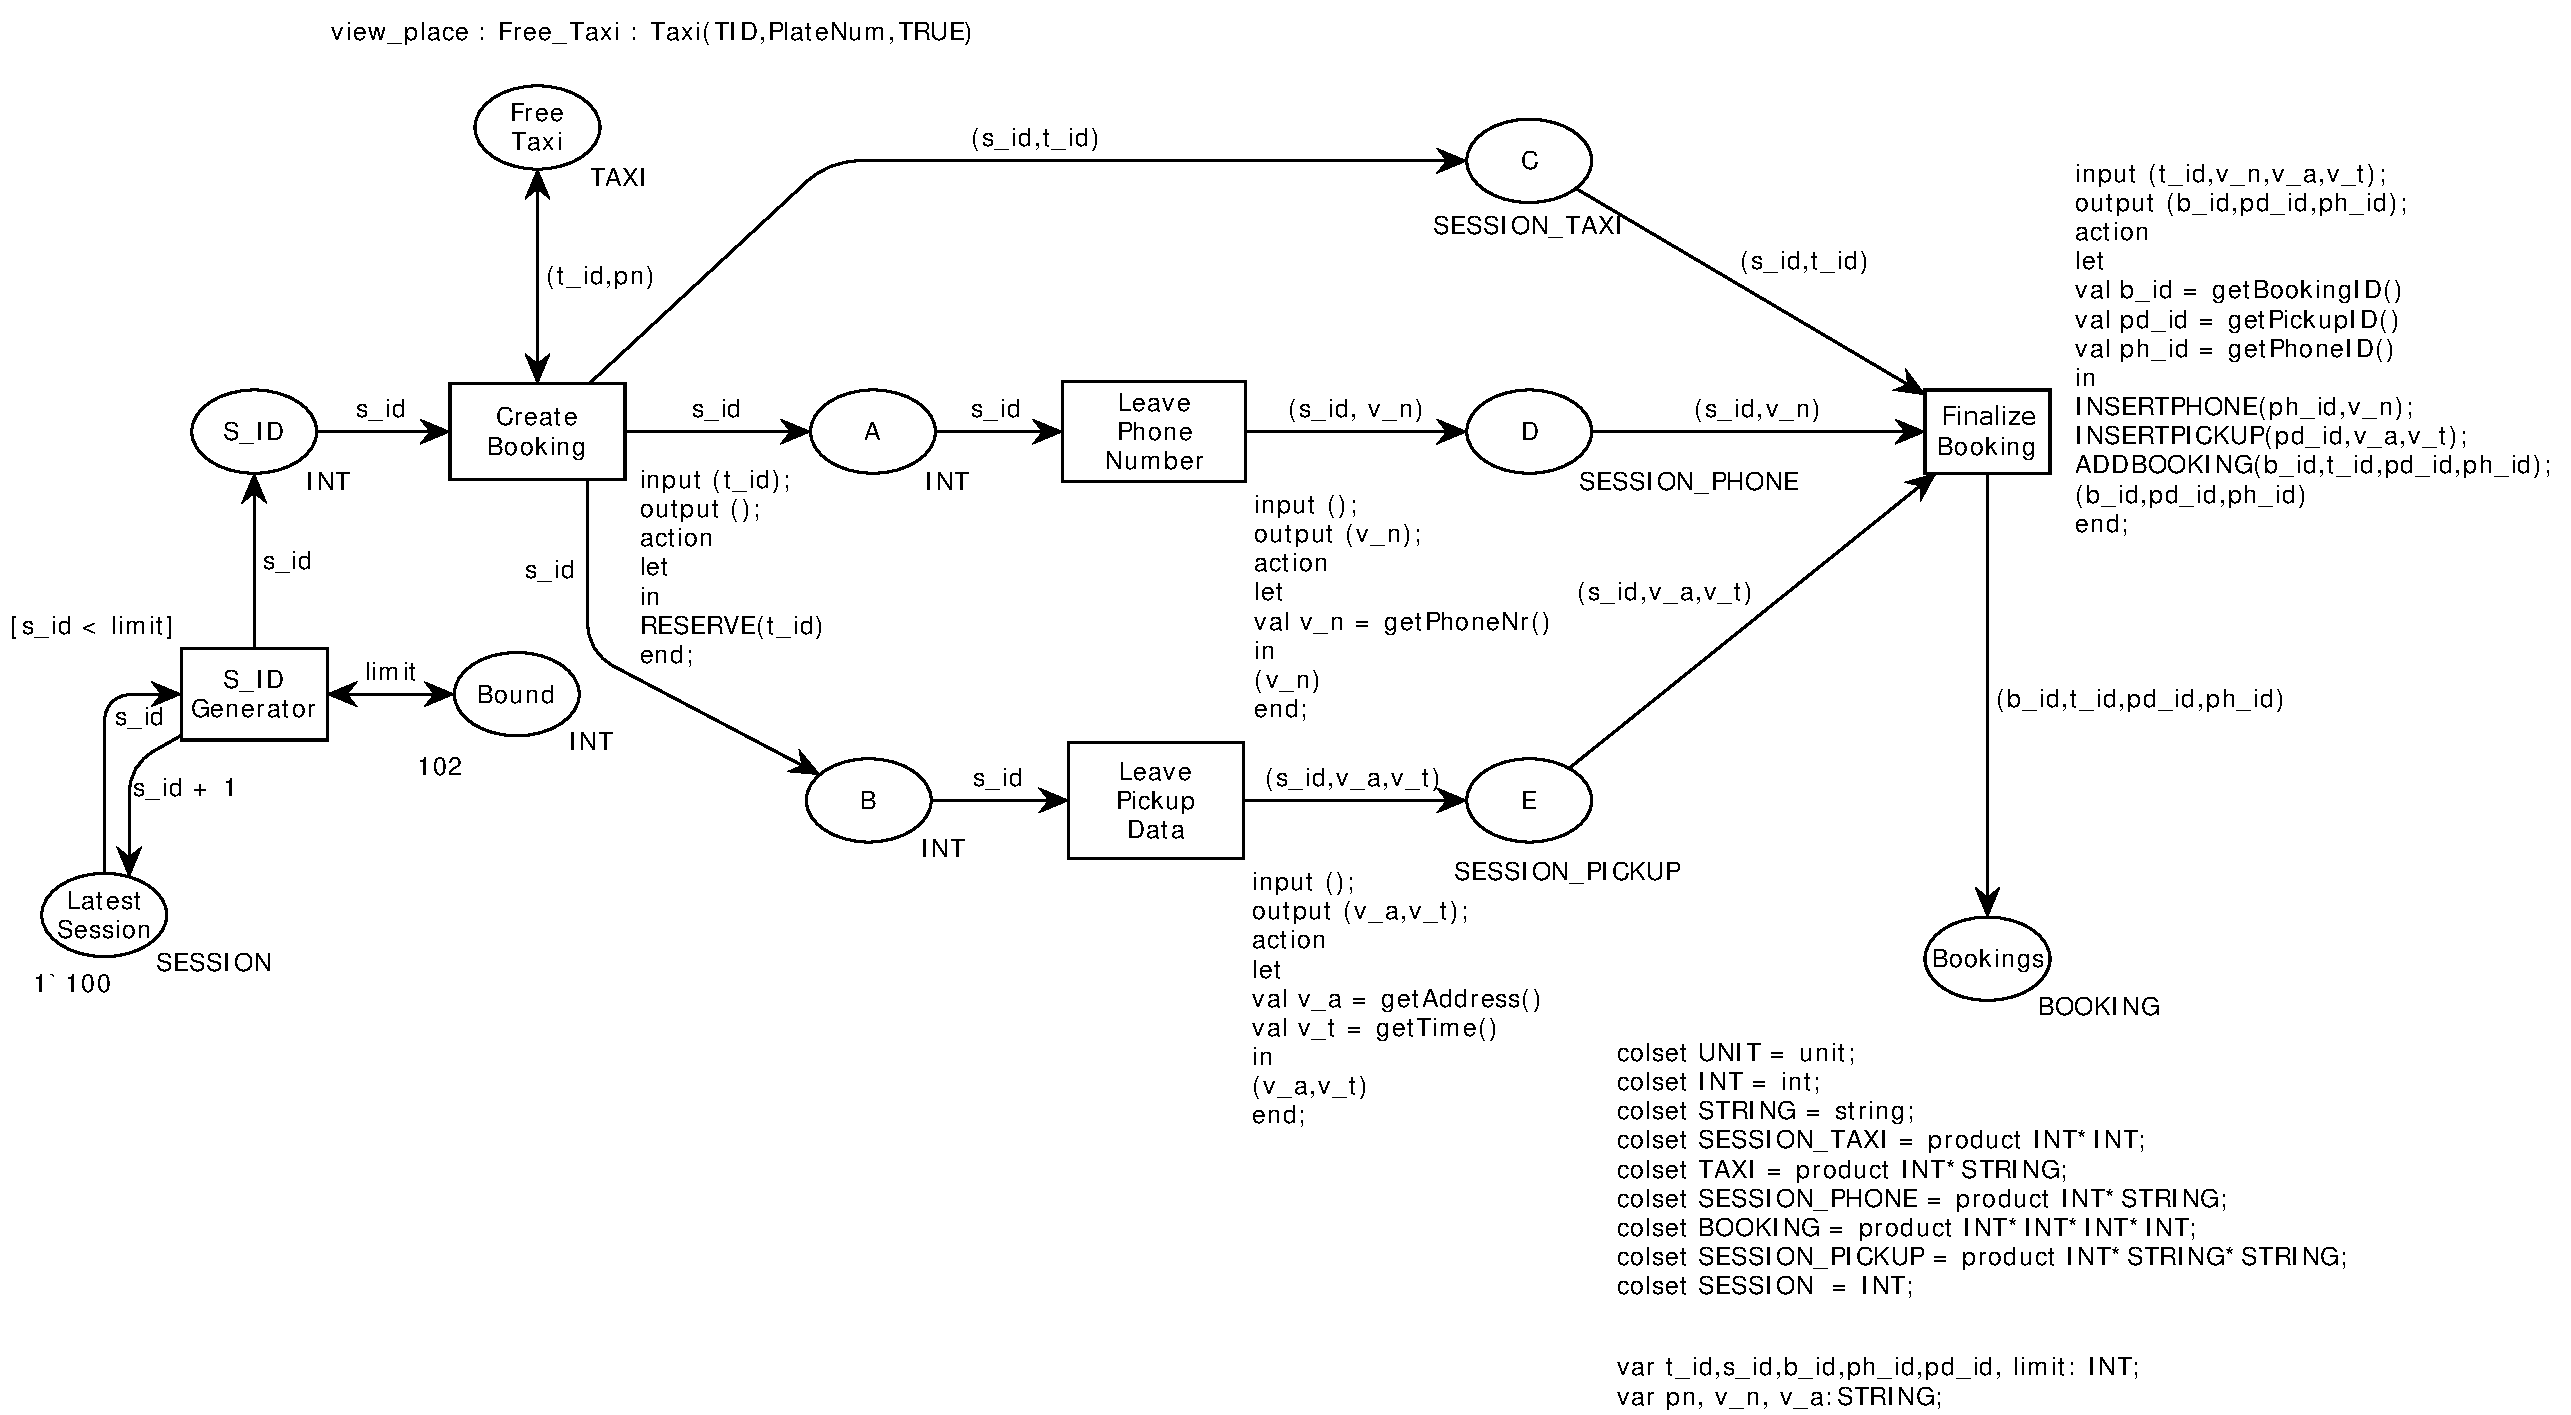
\includegraphics[scale = 0.33]{DBN_CPNTools_Taxi_Example.pdf}
	\caption{A db-net representing the taxi booking process modelled in CPN Tools}
	\label{fig:DBN_CPNTools_Taxi_Example}
\end{figure}

\subparagraph*{\textnormal{The major components in the DB-Nets are view places, read arcs, action transitions, the data logic layer and the data acquisition for fresh variables. Using these we could interact with the persistence layer. The execution semantics of CPNs can be applied over DBN. Additionally, after occurrence of every step, the view places need to be refreshed, e.g. the view place $\mathit{Free\ Taxi}$ needs to be updated when a step occurs in the net.}}

\subparagraph*{\textnormal{In the later chapters, we will see the development and working of the DB-Nets extension for CPN Tools.}}



\appendix
\chapter{Technical Specifications}
This chapter contains the exact specifications of the FUB-CS Dissertation Style.

\paragraph*{Page dimensions}
By default, the FUB-CS Dissertation Style uses the options
\verb|twoside|, \verb|a4paper| and \verb|12pt|.
The left and right margins are equal, as are the top and bottom margins.
\\[\baselineskip]
\begin{tabular}{|c|c|c|c|c|c|}\hline
Font Size &  Text   &  Text   & Height incl.& Left/Right & Top/Bottom \\
          &  Width  &  Height &  Head/Foot  &   Margin   & Margin     \\ \hline
 10 pt    &  121 mm &  182 mm &  201 mm     &  44.5 mm   &  57.3 mm   \\
 11 pt    &  133 mm &  200 mm &  222 mm     &  38.4 mm   &  45.2 mm   \\
 12 pt    &  145 mm &  218 mm &  242 mm     &  32.4 mm   &  33.1 mm   \\
12 pt (81\%)& 118 mm & 177 mm &  196 mm     &  25.7 mm   &  26.8 mm   \\ \hline
\end{tabular}

\paragraph*{The page head and foot}
Left-hand pages have the page-number in the upper left corner,
and the italized non-uppercase current chapter title in the upper right corner.
Right-hand pages have the page-number in the upper right corner,
and the italized non-uppercase current section title in the upper left corner.
If the \verb|\cleardoublepage| command causes a left-hand page to be empty,
that page will have neither page number nor page head.

\paragraph*{The chapter head}
By default, the FUB-CS Dissertation Style uses the option \verb|openright|.
With this option, chapters always start on a right-hand page
(using the \verb|\cleardoublepage| command).
The first page of a chapter has the pagenumber in the page foot,
and an empty page head.
Each chapter starts with
a blank space (18 pt high at a 12 pt fontsize),
the left-aligned boldfaced \verb|Large|-sized chapternumber,
a horizontal line,
the right-aligned boldfaced \verb|LARGE|-sized chaptertitle,
and another blank space (120 pt high at a 12 pt fontsize).

As mentioned in Chapter 2, you can change this with the fancy chapter option.

\paragraph*{Sectioning commands}
The commands \verb|\thebibliography| and \verb|\theindex| now
produce an entry in the table of contents.
The new sectioning commands \verb|\thesymbols|, \verb|\acknowledgements|,
\verb|\riassunto|, \verb|\zusammenfassung|, \verb|\abstract| and \verb|\curriculum| are defined.
All sectioning commands now produce non-uppercased page heads.

\paragraph*{Theorem-like environments}
All theorem-like environments begin with the number in bold-faced type,
`theorem' (or similar) in small caps,
and the optional argument (if any) in a normal fonttype.
The theorem-like environments
\verb|\theorem|,
\verb|\conjecture|,
\verb|\lemma|
\verb|\proposition| and
\verb|\corollary|
are predefined and have italicized text.
The theorem-like environments
\verb|\definition|,
\verb|\remark|,
\verb|\example|,
\verb|\convention|,
\verb|\fact| and
\verb|\question|
are predefined and have non-italicized text.
All predefined theorem-like environments are numbered consecutively,
within each section.

\paragraph*{Miscellaneous}
The \verb|fubcsdiss| class loads the \verb|graphicx| package,
and defines the commands 
\verb|\fubcslogo| and \verb|\fubcsnotextlogo|.
On systems where the \verb|graphicx| package is not available, you
can use the \verb|fubcsdiss-epsfig| class, which loads the
\verb|epsfig| package instead. This package is not suitable for
use in conjunction with \verb|pdflatex| however.



%%  \include the `end matter'

%\bibliographystyle{plain}
\begin{thebibliography}{XX}
\small
\bibitem{Comment}
According to FUB-CS standards a chapter containing bibliographic
references should always be included in your dissertation.
It is specified by:
\begin{verbatim}
  \begin{thebibliography}{XX}
    <your list of \bibitems>
  \end{thebibliography}
\end{verbatim}

\bibitem{Comment}
If you do not want numbers, then you can you can use, for instance, the very nice and powerful \texttt{natbib} package and have the references listed like the four below (and many options to vary citation in the text), or manually specify something like
\begin{verbatim}
\bibitem[L94]{Lamport}
\end{verbatim}
in your bibliography list to get \verb|[L94]| both in the text and between the square brackets in the bibliography. 

\bibitem[L94]{Lamport}
Lamport, L. {\em \LaTeX{} User's Guide \& Reference
Manual\/}, Addison-Wesley Publishing Company, Reading, Mass. 1986, 1994.

\bibitem[PR04]{Poggi04}
Poggi, A., Ruzzi, M. Filling the gap between data federation and data integration. In: di Pula, S.M. (ed.): \emph{Proceedings of the 12th Italian Symposium on Advanced Database Systems}, Cagliari, Italy. 2004. pp270-281.

\bibitem[PS06]{Pontow06}
	Pontow, C., Schubert, R. A mathematical analysis of theories of parthood. \emph{Data \& Knowledge Engineering}, 2006, 59:107-138.

\bibitem[Popper1996]{Popper96}
	Popper, K.R. \emph{The myth of the framework -- in defence of science and rationality}. London: Routledge. 1996. 229p.

\end{thebibliography}



\begin{theindex}
By preference, your dissertation\linebreak
should contain an index. Instructions
on how to produce an index can be
found on pages 77--79 of the
 \LaTeX\ manual. You may specify
an index as follows:\\[2ex]
\verb|  \begin{theindex}|\\
\verb|    <your list of entries>|\\
\verb|  \end{theindex}|
\end{theindex}


\begin{thesymbols}
This is an optional chapter containing a list of symbols that
you use. It is specified by:\\[2ex]
\verb|  \begin{thesymbols}|\\
\verb|    <your list of symbols>|\\
\verb|  \end{thesymbols}|
\end{thesymbols}

%\riassunto
According to FUB regulations (???), a chapter containing a summary in Italian of your dissertation should always be included.
It is specified by:
\begin{verbatim}
  \riassunto
    <your Riassunto>
\end{verbatim}
 %%%%%%%% optional
%\zusammenfassung
According to FUB regulations (???), a chapter containing a summary in German of your dissertation should always be included.
It is specified by:
\begin{verbatim}
\zusammenfassung
      <your Zusammenfassung >
\end{verbatim}
 %%%%%%%% optional
\curriculum
This is an optional chapter containing your Curriculum Vitae as brief ($\pm$ half a page) text, and add your publications in reverse chronological order spanning the years of doing your PhD.
It is specified as follows:
\begin{verbatim}
  \curriculum
    <your CV>
\end{verbatim}



%%  finally, \include the list of previous FUB-CS dissertations

\cleardoublepage % if you are so inclined
\pagestyle{empty}

\noindent
\begin{center}
\textbf{Titles in the FUB-CS Dissertation Series}\\
Collana di Tesi\\
{\em Reihe von Doktorarbeiten}
\par\vspace {1cm}
\end{center}

\newcommand{\fubcspublication}[3]{\item[FUB-CS #1: ]{\bf #2}\\{\em #3}}

\begin{list}{}{ \settowidth{\leftmargin}{ILL}
		\setlength{\rightmargin}{0in}
		\setlength{\labelwidth}{\leftmargin}
		\setlength{\labelsep}{0in}
}

\fubcspublication{DS-2008-01}{Catharina Maria Keet}{A Formal Theory of Granularity}
\fubcspublication{DS-2008-02}{Bruno Rossi}{Towards a Simulation Model including Network Externalities in Free/Libre Open Source Software (FLOSS) Adoption}
\fubcspublication{DS-2008-03}{Dino Seppi}{Prosody in Automatic Speech Processing}

\end{list}

\clearpage
\mbox{ }
\newpage

 %PERSONALIZE that is: make sure you have the latest list.
%{\pagestyle{empty}
\normalsize
\setlength\columnsep{20pt}
%      \columnseprule \z@
 %  \columnsep 35\p@
\par\vskip 1cm
%\begin{backsummary} %add later, see also fubdiss2.cls
   \twocolumn[{\Large FUB CS Diss Style}\\  %%PERSONALIZE
\textsl{any subtitle goes here}\vspace{8mm}] 		%PERSONALIZE

your summary of about 1 column goes\\
your summary of about 1 column goes here\\
your summary of about 1 column goes here\\
your summary of about 1 column goes here\\
your summary of about 1 column goes here\\
your summary of about 1 column goes here\\
your summary of about 1 column goes here\\
your summary of about 1 column goes here\\
your summary of about 1 column goes here\\
your summary of about 1 column goes here\\
your summary of about 1 column goes here\\
your summary of about 1 column goes here\\
your summary of about 1 column goes here\\
your summary of about 1 column goes here\\
your summary of about 1 column goes here\\
your summary of about 1 column goes here\\
your summary of about 1 column goes here\\
your summary of about 1 column goes here\\
your summary of about 1 column goes here\\
your summary of about 1 column goes here\\
your summary of about 1 column goes here\\
your summary of about 1 column goes here\\
your summary of about 1 column goes here\\
your summary of about 1 column goes here\\
your summary of about 1 column goes here\\
your summary of about 1 column goes here\\
your summary of about 1 column goes here\\
your summary of about 1 column goes here\\
your summary of about 1 column goes here\\
your summary of about 1 column goes here\\
your summary of about 1 column goes here\\
your summary of about 1 column goes here\\
your summary of about 1 column goes here\\
your summary of about 1 column goes here\\
your summary of about 1 column goes here\\
your summary of about 1 column goes here\\
your summary of about 1 column goes here\\
your summary of about 1 column goes here\\
your summary of about 1 column goes here\\
your summary of about 1 column goes here\\
your summary of about 1 column goes here\\
your summary of about 1 column goes here\\
your summary of about 1 column goes here\\
your summary of about 1 column goes here\\
your summary of about 1 column goes here\\
and balance it out a bit so that the logo is somewhere in the middle. alternatively, there is a 
\begin{verbatim}
\begin{backsummary} 
your summary goes here. 
see also fubdiss2.cls
\end{backsummary}
\end{verbatim}
%\end{backsummary}
\begin{center}
%\par\vspace {2cm}
\par\vspace {3.5cm}
\noindent%
\fublogo{7cm}
\end{center}
\vfill

%Copyright and accreditation stuff, plus ISBN
%
\noindent%
%\fubcslogo{5cm}\\
% Copyright: put your name here
\hfill Copyright \copyright\ 200x by John B. Goode\\[1ex] %PERSONALIZE
% Cover design, if your cover was designed by someone else
%Cover design by Mickey Mouse.\\                       %PERSONALIZE
%Maybe some additional info on the production of the dissertation.
%Don't forget your printing shop
\noindent \mbox{ } \hfill Printed and bound by DigiPrint\\[2ex]           %PERSONALIZE
%ISBN number: ask your faculty library how to obtain one
%\noindent \mbox{ } \hfill ISBN: 90--XXXX--XXX--X                              %PERSONALIZE
} 

%%%%%%%%%%%%%%%%%%%%%%%END of BACK MATTER%%%%%%%%%%%%%%%%%%%%%%%%%%%
 % for a thesis with a back-flap summary
%% This is the standard `front matter' to be used with the illcdiss.cls
%% Latex2e document class or the illc_diss.sty Latex2.09 style file
%%
%% Author: Maarten de Rijke
%% Current maintainer: Marco Vervoort
%%
%% Version: July, 2001
%%
%% MAKE SURE THAT THE FILE HAS BEEN PERSONALIZED BEFORE YOU
%% PRINT AND SHIP THE FINAL VERSION.  YOU CAN FIND ITEMS THAT NEED
%% TO BE PERSONALIZED BY SEARCHING FOR THE STRING ``%PERSONALIZE''
%%
%%
%%first of all the cover.
{\pagestyle{empty}
%\newcommand{\printtitle}{%
%{\Huge\bf The FUB-CS Dissertation\\[0.8cm] Style}}    %PERSONALIZE

%%the second page: the `illc pagina'
\clearpage
\par\vskip 2cm
\begin{center}
\par\vspace {2cm}
%\textbf{FUB-CS Dissertation Series DS-200X-NN}                 %PERSONALIZE
%\par\vspace {1cm}
%\noindent%
\fublogo{14cm}
\end{center}

\vfill

%Copyright and accreditation stuff, plus ISBN
%
\noindent%
%\fubcslogo{5cm}\\
% Copyright: put your name here
Copyright \copyright\ 2017 by Aman Sinha\\[2ex] %PERSONALIZE
% Cover design, if your cover was designed by someone else
%Cover design by ------.\\                       %PERSONALIZE
%Maybe some additional info on the production of the dissertation.
%Don't forget your printing shop
Printed and bound by your printer.\\[2ex]           %PERSONALIZE
%ISBN number: ask your faculty library how to obtain one
ISBN: 90--XXXX--XXX--X                              %PERSONALIZE

% Dedication, table of contents and acknowledgements
% are handled in the main file

\clearpage
} % Back to \pagestyle{plain}

%%%%%%%%%%%%%%%%%%%%%%%END of BACK MATTER%%%%%%%%%%%%%%%%%%%%%%%%%%%
 %or take this one for a fairly plain back cover
 
\end{document}